%======================================================================
%  CSE 450 Capstone Project -- Report
%  Department of Computer Science and Engineering, BUET
%
%  Build:  latexmk -pdf template.tex   (or Overleaf, compiler: pdfLaTeX)
%======================================================================
\documentclass[12pt,a4paper,oneside]{report}
\usepackage{cse-capstone}

% TikZ (already pulled in by pgfgantt) is used for the architecture and
% skill-graph figures in Chapter 4.
\usetikzlibrary{arrows.meta,positioning,fit,backgrounds}

% ---------------------------------------------------------------------
\newcommand{\ProjectTitle}{ATLAS: An Adaptive Tutoring System using
Bayesian Knowledge Tracing over a Prerequisite Skill Graph}
% TODO: replace with your actual session, e.g. Session 2021--2022
\newcommand{\Session}{Session 2026--20X27}
% TODO: replace with your actual submission month and year
\newcommand{\SubmissionDate}{September 2026}
% TODO: replace with your actual supervisor's name and designation
\newcommand{\Supervisors}{%
  Dr. Md. Shariful Islam Bhuyan\\
  Associate Professor, Department of CSE, BUET}
% Team members are listed in frontmatter/titlepage.tex and declaration.tex
% ---------------------------------------------------------------------

\hypersetup{pdftitle={\ProjectTitle}}

\begin{document}

\pagenumbering{gobble}
\thispagestyle{empty}
\begin{center}

{\large CSE450 Capstone Project Report}

\vspace*{\stretch{2}}
{\LARGE\bfseries \ProjectTitle}

\vspace*{\stretch{4}}
{\large Submitted by}\\[10pt]
% TODO: replace the five rows below with the real names and student IDs.
% Git history identifies five contributors; the IDs visible in commit
% metadata were 2105066, 2105094 and 2105104.
\begin{tabular}{ll}
  Sakif Naieb Raiyan & 2105065 \\
  Sayaad Muzahid Masfi & 2105066 \\
  Aurchi Chowdhury & 2105083 \\
  Omar Abdur Razzaque & 2105094 \\
  Rubaiyat - E- Zaman & 2105104
\end{tabular}

\vspace*{\stretch{3}}
{\large Supervised by}\\[10pt]
\Supervisors

\vspace*{\stretch{3}}

\includegraphics[width=30mm]{buet_logo.png}\\[8pt]
\textbf{Department of Computer Science and Engineering}\\
{\large\bfseries Bangladesh University of Engineering and Technology}\\
Dhaka, Bangladesh

\vspace*{\stretch{1}}
\Session\\
\SubmissionDate

\end{center}
\clearpage

\pagenumbering{roman}
\begin{center}
  {\Large\bfseries CANDIDATES' DECLARATION}
\end{center}
\addcontentsline{toc}{chapter}{Candidates' Declaration}

\vspace{20pt}
We declare that the work presented in this report, titled
``\ProjectTitle'', is the outcome of the engineering work carried out by us
under the supervision named on the title page.

All prior work, third-party code, libraries, data, copyrighted material, and
tools used in the project have been properly acknowledged. Any use of
generative AI tools has been disclosed. We accept accountability and
responsibility for the accuracy and integrity of this report and for our
individual contributions to the project.

\vspace{15mm}
% TODO: replace with the real names and IDs, matching frontmatter/titlepage.tex.
\begin{tabular}{>{\raggedright\arraybackslash}p{0.45\textwidth} >{\raggedright\arraybackslash}p{0.45\textwidth}}
  \rule{0.4\textwidth}{0.4pt} & \rule{0.4\textwidth}{0.4pt} \\
  Sakif Naieb Raiyan (2105065) & Sayaad Muzahid Masfi (2105066) \\[15mm]
  \rule{0.4\textwidth}{0.4pt} & \rule{0.4\textwidth}{0.4pt} \\
  Aurchi Chowdhury (2105083) & Omar Abdur Razzaque (2105094) \\[15mm]
  \rule{0.4\textwidth}{0.4pt} & \\
  Rubaiyat - E- Zaman (2105104) &
\end{tabular}
\clearpage

\chapter*{ACKNOWLEDGEMENT}
\addcontentsline{toc}{chapter}{Acknowledgement}

We thank our supervisor for the guidance and critical questioning that shaped
this project, and in particular for pressing us on the point that ultimately
defined the work: that an adaptive tutor is only as good as the knowledge
structure underneath it, and that a shallow skill map cannot be rescued by a
sophisticated inference algorithm sitting on top of it.

We are grateful to the Department of Computer Science and Engineering, BUET,
for the CSE 450 Capstone framework, which gave this work both its scope and its
deadlines.

The subject-matter content of this system is drawn from standard Higher
Secondary Certificate (HSC) textbooks and past admission-test question banks
for Bangladeshi engineering universities. We acknowledge the authors and
publishers of that material; it is used here strictly as source material for an
academic prototype and is not redistributed as part of the system.

% TODO: Add personal acknowledgements here -- specific teachers or domain
% experts who reviewed chemistry or physics content, friends or juniors who
% tested the interface, and anyone outside the team who gave feedback. The
% report is stronger if these are named concretely rather than generically.

\clearpage

\chapter*{ABSTRACT}
\addcontentsline{toc}{chapter}{Abstract}
\begingroup
\small
\setlength{\parskip}{1.5mm}

Every year a large cohort of Bangladeshi students prepares for the engineering
university admission tests (BUET, KUET, RUET, CUET) by working through
undifferentiated question banks. A student who repeatedly fails questions on
integration by parts is rarely told that the actual gap is algebraic
manipulation two levels below; coaching centres cannot diagnose at that
granularity at scale, and existing digital platforms largely serve the same
fixed content to everyone. The engineering problem is therefore one of
inference under uncertainty: from a sparse, noisy sequence of multiple-choice
responses, locate a learner's knowledge frontier precisely enough to act on it.

This report presents ATLAS, an adaptive tutoring system that models a learner's
latent mastery with Bayesian Knowledge Tracing (BKT) over a directed acyclic
graph (DAG) of prerequisite relations between granular skills. Three extensions
to textbook BKT carry the design. First, the guess and slip parameters are
conditioned on the Bloom's Taxonomy level of the question, so that a correct
answer on a recall item and a correct answer on an analysis item update belief
by different amounts. Second, a correct response propagates upward through the
prerequisite graph, raising every ancestor to at least the descendant's
posterior, since demonstrating a dependent skill is evidence for the skills it
depends on. Third, a skill's learning-rate parameter is gated conjunctively:
it rises only when \emph{all} of its direct prerequisites are mastered,
preventing a learner from appearing to advance past an unmastered foundation.
An adaptive diagnostic selects each next question by a balanced-volume
heuristic over untested ancestors and descendants, at one Bloom level above the
learner's current estimated band.

The system was built as a FastAPI backend, a React frontend rendering Bangla
text with embedded \LaTeX{} mathematics, and a PostgreSQL (Supabase) store. A
retrieval-augmented generation pipeline over six HSC textbooks (4{,}474 parsed
question records) produces the question bank, with a two-model
generate-then-verify design in which a second model blind-re-solves each
generated item before it is accepted. The knowledge structure itself was the
dominant engineering effort: an initial 430-skill ontology derived from a
sample of the corpus proved too sparse to support the gating policy, and was
rebuilt from the full corpus into 1{,}688 skills and 1{,}743 prerequisite edges
covering all 183 syllabus topics, validated as an acyclic graph of depth 9 with
no isolated skills.

Verification is structural and functional rather than empirical: an 18-check
end-to-end harness exercises the diagnostic, mastery propagation, the
ancestor-ordering invariant and prerequisite spillover against an in-memory
database stand-in, and passes completely; the ontology passes an automated
structural validator with zero errors. The system has not yet been evaluated
with human learners, and establishing that its mastery estimates predict real
performance remains the principal item of future work.

\vspace{12pt}
\noindent\textbf{Keywords:} Bayesian Knowledge Tracing; adaptive learning;
prerequisite graph; Bloom's Taxonomy; intelligent tutoring systems;
retrieval-augmented question generation
\endgroup
\clearpage

\tableofcontents
\listoffigures
\listoftables

\clearpage
\pagenumbering{arabic}
% Chapter 1 -- Rubric: PO1 (1.1), PO2 (problem identification), PO3 (3.2 objectives)
\chapter{Problem Identification and Formulation}
\label{ch:problem}

\section{Background and Motivation}
\label{sec:background}

Admission to the engineering universities of Bangladesh --- BUET, KUET, RUET
and CUET --- is decided by a single competitive examination taken after the
Higher Secondary Certificate (HSC). The test covers Mathematics, Physics and
Chemistry, and the ratio of candidates to available seats is severe enough that
preparation is effectively a year-long full-time activity for those who attempt
it. The dominant preparation method is volume: a student buys one or more
question banks compiled from previous years' papers and works through them,
usually alongside coaching-centre classes that move at a fixed pace through a
fixed syllabus.

This method has a structural weakness that has nothing to do with effort. When
a student fails a question, the question bank tells them the correct answer; it
does not tell them \emph{why} they failed. A wrong answer on a problem
requiring integration by parts may indicate that the student does not recognise
when the technique applies, or cannot choose $u$ and $dv$ correctly, or chose
them correctly but made an algebraic error in the resulting simpler integral,
or does not know the derivative of the function involved. These are four
different deficits requiring four different remedies, and they are invisible in
a score. A human tutor localises them by watching the student work --- which is
precisely what one-to-one tutoring is effective at, and precisely what does not
scale to a national cohort \cite{vanlehn2011relative}.

The consequence is misallocated study time. A student who does not know which
of their foundations is weak has no rational basis for choosing what to study
next, and defaults to either linear syllabus coverage or to practising the
topics where failure is most visible --- often the topics \emph{downstream} of
the actual gap. Time spent re-attempting integration problems does not repair
an algebra deficit; it merely produces repeated failure on the same
prerequisite, which is both inefficient and demoralising.

What is needed is a system that infers, from the student's own answers, where
in the structure of the subject their knowledge stops --- and then selects the
next question at that frontier rather than at the point in the syllabus the
calendar happens to have reached.

\section{Problem Statement}
\label{sec:problem-statement}

\textbf{Problem.} Given a learner and a sequence of their responses to
multiple-choice questions, estimate the learner's mastery of every skill in a
subject domain, and select the next question so as to localise and repair the
learner's knowledge frontier.

Formulated in engineering terms:

\begin{itemize}
  \item \textbf{Entities.} A set of \emph{skills} $S = \{s_1,\dots,s_n\}$, each
    an atomic, independently testable unit of knowledge or procedure, annotated
    with one Bloom's Taxonomy cognitive level. A set of directed
    \emph{prerequisite} edges $E \subseteq S \times S$, where $(s_i,s_j) \in E$
    means $s_i$ must be held before $s_j$ is reachable. A bank of questions,
    each tagged with the skill it tests, its Bloom level and its topic. A set of
    learners.
  \item \textbf{Inputs.} For a learner $u$, an observed sequence of binary
    outcomes $(q_1,c_1),(q_2,c_2),\dots$ where $q_t$ is the question served at
    step $t$ and $c_t \in \{\text{correct},\text{incorrect}\}$.
  \item \textbf{Latent state.} For each skill, $P(L_{u,s}) \in [0,1]$, the
    probability that learner $u$ has learned skill $s$. This is never observed
    directly; it must be inferred from noisy evidence.
  \item \textbf{Outputs.} (i) The posterior $P(L_{u,s})$ for all $s \in S$
    after each response; (ii) the identity of the next question to serve.
  \item \textbf{Quantities to be guaranteed.} The graph $(S,E)$ must be acyclic,
    or the notion of ``prerequisite'' is incoherent and propagation does not
    terminate. Mastery estimates must respect the graph: no skill may be
    credited as mastered while an ancestor it depends on is estimated as
    unmastered. Question selection must terminate even when the bank has no
    item matching the ideal specification.
  \item \textbf{Assumptions.} Responses are conditionally independent given the
    latent state; a learner does not forget within a session (no decay term);
    each question tests primarily one skill; the prerequisite structure is the
    same for all learners.
\end{itemize}

\noindent\textbf{Engineering knowledge demanded.} The formulation above is not
solvable by routine application of standard components. It requires: probability
theory and Bayesian inference (the latent-state update); graph theory (acyclicity
checking, topological ordering, transitive reduction, ancestor traversal);
algorithm design (the question-selection heuristic and its fallback ladder);
database design under referential constraints; the pedagogical literature on
knowledge tracing and cognitive taxonomies, which supplies the model family and
the level annotation scheme; and, for the content pipeline, applied natural
language processing --- retrieval-augmented generation, embedding-based
retrieval, and the validation of machine-generated assessment items.

\section{Complexity of the Problem}
\label{sec:complexity}
A complex engineering problem must have characteristic P1 and some or all of
P2--P7 (\Cref{tab:complexity}). P1 requires in-depth knowledge at the level
of one or more of the knowledge profiles K3--K8 listed in
\Cref{tab:knowledge-profile}.

% Rendered as a longtable (not a float) so it flows across pages at readable
% size instead of being squeezed onto one rotated page.
\setlength{\LTcapwidth}{\textwidth}
{\small\setstretch{1.1}
\begin{longtable}{@{}p{11mm}p{56mm}p{\dimexpr\textwidth-11mm-56mm-4\tabcolsep\relax}@{}}
  \caption{Complex engineering problem characteristics (P1--P7) and evidence from this project}
  \label{tab:complexity}\\
    \toprule
    Code & Definition & Evidence from this project \\
    \midrule
  \endfirsthead
    \multicolumn{3}{@{}l}{\small\itshape \tablename~\thetable{} --- continued from previous page}\\[2pt]
    \toprule
    Code & Definition & Evidence from this project \\
    \midrule
  \endhead
    \midrule
    \multicolumn{3}{r@{}}{\small\itshape continued on next page}\\
  \endfoot
    \bottomrule
  \endlastfoot
    P1 & \textbf{Depth of knowledge required.} Cannot be resolved without in-depth engineering knowledge at the level of one or more of K3, K4, K5, K6, or K8, which allows a fundamentals-based, first-principles analytical approach. &
    \textbf{K3, K4, K5, K8.} K3: the Bayesian update is derived from first principles, not called from a library --- the posterior and transition equations are implemented directly (\Cref{sec:bkt-model}). K4: knowledge tracing and cognitive-taxonomy literature supplies the model family \cite{corbett1995knowledge,anderson2001revised}. K5: the DAG, its acyclicity guarantee and transitive reduction are what make the gating policy implementable. K8: the design engages directly with the research literature on BKT variants \cite{baker2008more,yudelson2013individualized,pardos2011kt} and on prerequisite-structured student models \cite{kaser2017dynamic}. \\
    P2 & \textbf{Range of conflicting requirements.} Involves wide-ranging or conflicting technical, engineering, and other issues. &
    Granularity conflicts with question-bank coverage: finer skills localise gaps better but multiply the items needed (the rebuilt ontology raised the generation space from $430\times6$ to $1{,}688\times6$ tuples). Diagnostic length conflicts with learner patience: 30 questions cannot cover 430 skills, forcing inference by propagation rather than measurement. Adaptivity conflicts with stability: an aggressive learning rate tracks change quickly but overreacts to a lucky guess. \Cref{sec:alternatives} resolves these explicitly. \\
    P3 & \textbf{Depth of analysis required.} Has no obvious solution and requires abstract thinking and originality in analysis to formulate suitable models. &
    Textbook BKT is per-skill and independent; it cannot express ``mastery of $s_j$ is impossible while $s_i$ is unmastered.'' Making it graph-aware required an original three-phase policy (Bloom-conditioned update, ancestor pull-up, conjunctive transition gating) that is not a published algorithm but a composition designed for this problem (\Cref{sec:mastery-policy}). \\
    P4 & \textbf{Familiarity of issues.} Involves infrequently encountered issues. &
    Bangla-language STEM content with embedded \LaTeX{} mathematics is outside the well-trodden path: it broke JSON escaping (a corruption affecting a measured 13.4\% of one generated batch), broke text rendering in the browser, and is poorly served by English-centric embedding models. \\
    P5 & \textbf{Extent of applicable codes.} Is outside problems encompassed by standards and codes of practice for professional engineering. &
    No standard governs what a ``skill'' is, how finely a syllabus should be decomposed, or when an automatically generated assessment item is fit to serve to a student. These decisions were made against explicit project-defined criteria (\Cref{sec:standards}) because no code of practice supplies them. \\
    P6 & \textbf{Extent of stakeholder involvement and conflicting requirements.} Involves diverse groups of stakeholders with widely varying needs. &
    Learners want the shortest path to a higher score; teachers want syllabus fidelity and correct content; the system's own policy wants maximal information per question. These pull in different directions --- the most informative question is often not the most encouraging one. \Cref{sec:requirements} tabulates the conflicts. \\
    P7 & \textbf{Interdependence.} Is a high-level problem including many component parts or sub-problems. &
    Five interdependent subsystems: the knowledge ontology, the inference engine, the question bank and its generation pipeline, the serving API, and the learner-facing interface. The ontology is upstream of all others --- its granularity determines what the engine can infer and what the generator must produce, which is why a sparse first ontology forced a full rebuild (\Cref{sec:ontology-rebuild}). \\
\end{longtable}}

\begin{table}[htbp]
  \centering
  \caption{Knowledge profiles referenced by P1}
  \label{tab:knowledge-profile}
  \begin{tabularx}{\textwidth}{lY}
    \toprule
    Code & Description \\
    \midrule
    K3 & A systematic, theory-based formulation of engineering fundamentals required in the engineering discipline. \\
    K4 & Engineering specialist knowledge that provides theoretical frameworks and bodies of knowledge for the accepted practice areas in the engineering discipline; much is at the forefront of the discipline. \\
    K5 & Knowledge that supports engineering design in a practice area. \\
    K6 & Knowledge of engineering practice (technology) in the practice areas in the engineering discipline. \\
    K8 & Engagement with selected knowledge in the research literature of the discipline. \\
    \bottomrule
  \end{tabularx}
\end{table}

\section{Project Objectives and Scope}
\label{sec:objectives}

\subsection{Objectives}

The project set the following verifiable objectives. \Cref{ch:evaluation}
evaluates the delivered system against each.

\begin{enumerate}[label=\textbf{O\arabic*.}, leftmargin=*]
  \item \textbf{Construct a prerequisite skill graph} for the HSC Mathematics,
    Physics and Chemistry syllabus at a granularity fine enough that a single
    node names one independently testable action, and verify that the graph is
    acyclic and free of isolated nodes.
  \item \textbf{Implement a knowledge-tracing engine} that maintains a
    per-learner, per-skill mastery estimate, updates it from each response by
    Bayesian inference, and conditions that inference on the cognitive level of
    the question.
  \item \textbf{Make the estimate graph-aware}, such that evidence propagates to
    prerequisite skills and no skill can be credited above an unmastered
    prerequisite.
  \item \textbf{Deliver an adaptive diagnostic} that localises a learner's
    frontier within a bounded number of questions (target 30) rather than
    testing every skill.
  \item \textbf{Deliver targeted practice} that drives a chosen topic to a
    defined mastery threshold and detects when repeated failure is caused by a
    missing prerequisite rather than by the topic itself.
  \item \textbf{Produce a question bank} aligned to the skill graph, in Bangla
    with correct mathematical typesetting, via an automated pipeline with a
    verification stage.
  \item \textbf{Deliver a usable web application} exposing the diagnostic,
    practice and a mastery view to a learner.
  \item \textbf{Verify the engine end to end} with an automated test harness that
    runs without external credentials.
\end{enumerate}

\subsection{Scope}

\textbf{Included:} the three admission-test subjects; multiple-choice items
with four options; a single-process web deployment sufficient for demonstration;
Bangla content with \LaTeX{} mathematics; English and Bangla interface text.

\textbf{Explicitly excluded:} written/subjective answer grading; handwriting or
image input; mobile-native applications; teacher-facing classroom analytics;
multi-tenant institutional deployment; live proctoring; and any claim of
improved examination outcomes, which would require a controlled study with human
participants that this project did not undertake (\Cref{sec:eval-limits}).

% Chapter 2 -- Rubric: PO1 (1.1), PO2 (research literature), feeds PO3 and PO11
\chapter{Preliminary Research}
\label{ch:research}

\section{Literature Review}
\label{sec:literature}

\subsection{Modelling what a learner knows}

The problem of inferring an unobservable knowledge state from observable
responses has a long history in intelligent tutoring systems. Bayesian
Knowledge Tracing (BKT), introduced by Corbett and Anderson
\cite{corbett1995knowledge}, remains the reference formulation: a skill's
mastery is a hidden binary variable, and four parameters govern its evolution
--- a prior $P(L_0)$, a learning rate $P(T)$, and two noise terms, the slip
probability $P(S)$ (knowing but answering wrongly) and the guess probability
$P(G)$ (not knowing but answering correctly). The model's durability comes from
the fact that these four parameters are interpretable to a teacher, which is not
true of most of its successors.

The literature has extended BKT along three axes that are directly relevant
here. The first is \emph{parameter individualisation}: Yudelson et al.
\cite{yudelson2013individualized} fit per-student parameters and report
improved predictive accuracy, establishing that treating all learners as
identical is a real source of error. The second is \emph{contextualisation of
noise}: Baker et al. \cite{baker2008more} estimate slip and guess per response
rather than per skill, on the argument that a guess on a four-option item is not
the same event as a guess on an open response. Pardos and Heffernan
\cite{pardos2011kt} make the related argument for item difficulty. The third is
\emph{structure between skills}: Käser et al. \cite{kaser2017dynamic} model
students with dynamic Bayesian networks in which skills are linked by
prerequisite relations, and report that exploiting that structure improves
prediction over independent per-skill models.

Competing model families exist. Learning Factors Analysis \cite{cen2006learning}
and Performance Factors Analysis \cite{pavlik2009performance} replace the
hidden-state formulation with logistic regression over counts of prior successes
and failures. Deep Knowledge Tracing \cite{piech2015deep} replaces it with a
recurrent neural network and reports substantial accuracy gains on large
datasets. These are relevant as alternatives considered
(\Cref{sec:alternatives}) but share a property that disqualified them here:
their internal state is not interpretable as ``this student has not mastered
this specific skill,'' which is exactly the output this system must produce in
order to act on it.

A separate and older tradition, knowledge space theory
\cite{doignon1985spaces,falmagne2011learning}, formalises a domain as a
partially ordered set of knowledge states and asks which questions most
efficiently locate a learner within it. This is the theoretical ancestor of the
prerequisite graph used here, and it supplies the central insight that a
well-structured domain permits assessment far shorter than the number of skills,
because observing one response constrains many states at once.

\subsection{Cognitive level as a modelling variable}

Bloom's taxonomy \cite{bloom1956taxonomy}, in its revised form
\cite{anderson2001revised}, classifies learning objectives into six ascending
cognitive levels from Remember to Create. Its use in tutoring systems is usually
editorial --- a way of labelling items --- rather than a variable inside the
student model. The observation this project builds on is that the taxonomy has a
direct probabilistic reading: a four-option recall question can be answered
correctly by chance far more easily than an analysis question, and a learner who
genuinely knows an analysis-level skill is more likely to slip on it through a
procedural error. That makes the Bloom level a natural conditioning variable for
$P(G)$ and $P(S)$, which is the refinement Baker et al. \cite{baker2008more}
argue for on empirical grounds but implemented from a pedagogical prior rather
than a fitted one.

Vygotsky's zone of proximal development \cite{vygotsky1978mind} supplies the
selection rule: instruction is most effective just beyond what the learner can
already do unaided. Translated into this system's terms, the next question
should sit one Bloom level above the learner's current estimated band --- which
is the rule the diagnostic implements.

\subsection{Automatic generation of assessment items}

Kurdi et al. \cite{kurdi2020systematic} survey automatic question generation for
education and report the field's persistent difficulty: generated items are
often syntactically fine but pedagogically hollow, and evaluation of their
quality is usually thin. Retrieval-augmented generation
\cite{lewis2020retrieval} addresses part of this by grounding generation in
retrieved source material rather than in model memory, which both improves
factual accuracy and ties items to a specific curriculum. Multilingual sentence
embeddings \cite{reimers2019sentence} make such retrieval feasible over a
non-English corpus.

\subsection{What the literature establishes, and what it leaves open}

Established: BKT is an adequate and interpretable model of per-skill mastery;
its noise parameters should not be uniform across items; prerequisite structure
between skills carries real predictive value; and short adaptive assessment is
possible when the domain is well structured.

Left open, and therefore the space this project works in: the literature
provides no standard method for \emph{constructing} a fine-grained prerequisite
graph for a specific national syllabus --- the graphs in published work are
either small, hand-built by domain experts, or learned from response data that
does not exist before a system is deployed. Nor does it settle how a
Bloom-conditioned, graph-propagating variant of BKT should behave when the
question bank is incomplete, which is the normal condition of a system built
before it has users.

\section{Existing Solutions and Technologies}
\label{sec:related}

\begin{table}[htbp]
  \centering
  \caption{Existing solutions surveyed, and their limitations for this problem}
  \label{tab:existing}
  \begin{tabularx}{\textwidth}{>{\hsize=0.6\hsize}Y>{\hsize=0.75\hsize}Y>{\hsize=1.65\hsize}Y}
    \toprule
    Category & Examples & Strengths and limitations for this problem \\
    \midrule
    Adaptive commercial platforms & ALEKS; Knewton-style adaptive engines &
    Strength: mature adaptive engines with knowledge-space foundations and
    demonstrated scale. Limitation: closed, licensed per seat, and built around
    Western curricula --- no HSC syllabus coverage, no Bangla content, and no
    ability to add either. \\
    Bangladeshi ed-tech platforms & 10 Minute School, Shikho and similar &
    Strength: strong local content, Bangla-first, priced for the local market,
    already trusted by the target cohort. Limitation: predominantly
    content-delivery and fixed mock tests; assessment reports a score per test
    or per chapter rather than inferring a per-skill knowledge state, so the
    student still has to decide what to study next. \\
    Generic quiz and spaced-repetition tools & Quizlet, Anki, Google Forms &
    Strength: free, simple, and effective for pure recall
    \cite{ebbinghaus1885memory}. Limitation: no model of prerequisite structure
    at all --- a card is either due or not due --- so they cannot diagnose
    \emph{why} an item was failed or redirect to an upstream deficit. \\
    Printed question banks and coaching centres & The incumbent method &
    Strength: authoritative content, human explanation, peer environment.
    Limitation: fixed pace for a heterogeneous room; diagnosis at the
    granularity of a chapter, not a skill; and the marginal cost of one-to-one
    attention is precisely what prevents it scaling
    \cite{vanlehn2011relative}. \\
    Open-source ITS frameworks & pyBKT and similar research toolkits &
    Strength: reference implementations of the model family, useful for
    validation. Limitation: libraries, not products --- they supply the
    inference but neither the ontology, the content, nor the serving layer,
    which is where the majority of this project's effort actually went. \\
    \bottomrule
  \end{tabularx}
\end{table}

\noindent\textbf{The gap.} No surveyed system combines (i) a fine-grained
prerequisite model of \emph{this} syllabus, (ii) inference that is interpretable
per skill and propagates across prerequisite structure, and (iii) Bangla content
with correct mathematical typesetting. Platforms that have the content lack the
model; platforms that have the model lack the content and the language. ATLAS
targets that intersection.

\section{Market and User Research}
\label{sec:market}

\textbf{User base.} The primary users are HSC-completing students in Bangladesh
preparing for engineering admission tests, typically in a concentrated period
between the HSC examination and the admission tests. Secondary users are
repeat candidates and students in the HSC years using the system for syllabus
practice rather than test preparation.

\textbf{What users do instead.} Current practice, established from the team's
own experience of the same examination and from the structure of the material
that dominates the market, is: solve past-paper compilations; attend coaching
classes; sit periodic mock tests that return a rank and a score. The gap this
leaves is diagnostic, not informational --- students do not lack content, they
lack a reliable answer to ``what should I study next?''

\textbf{Demand characteristics.} Willingness to spend on preparation is
demonstrably high, since coaching enrolment is close to universal among serious
candidates, but willingness to spend on \emph{software} is low; the realistic
price point for a digital tool is at or near zero for the student, with revenue
arriving through institutions if at all (\Cref{sec:economics}).

\textbf{Evidence and its limits.} The characterisation above is grounded in the
team's direct familiarity with the examination and an informal survey of
available platforms and printed material. It is \emph{not} grounded in a
structured survey of prospective users with a defined sample; no such study was
conducted. This is a genuine weakness of the project's user research, stated
here rather than obscured, and \Cref{sec:conclusion} lists it as future work.
% TODO (optional but recommended): if the team can run even a small structured
% survey of 30--50 candidates before submission, replace the paragraph above
% with real figures -- it converts the weakest section of this chapter into a
% strength.

\section{Feasibility Study}
\label{sec:feasibility}

\textbf{Technical.} Feasible, and demonstrated. The inference model is
computationally trivial (a constant-time update per response plus an ancestor
traversal bounded by graph depth, measured at 9). The content pipeline was the
real technical risk: it depends on a large language model producing correct
Bangla mathematical content at scale. That risk was retired empirically --- an
initial attempt using local models on CPU hardware proved infeasible on
throughput grounds and was abandoned, and a hosted API with a
generate-then-verify design was substituted successfully
(\Cref{sec:generation-pipeline}).

\textbf{Economic.} Feasible at prototype scale at essentially zero marginal
cost: every service used (database, model API, hosting) has a free tier adequate
for development and demonstration. It is \emph{not} feasible to assume those
free tiers extend to production; \Cref{sec:economics} models the real operating
cost.

\textbf{Operational.} The adoption question is the binding one. The system asks
a student to spend 30 questions on a diagnostic before it gives them anything,
which is a real cost to a user under time pressure who is accustomed to
immediate practice. Mitigation is to make the diagnostic itself feel like
practice --- it serves genuine past-paper-style questions, not artificial
calibration items.

\textbf{Legal and regulatory.} Feasible with attention. The system stores
learner performance data, which is personal data; the source content is drawn
from copyrighted textbooks and question banks, which constrains redistribution.
Both are addressed in \Cref{sec:standards} and \Cref{sec:ip}.

\textbf{Conclusion.} The project is feasible, and the principal assumption it
depends on is that a machine-constructed skill ontology, validated structurally
but not yet by domain experts, is an adequate foundation for the inference built
on top of it. That assumption is explicitly flagged as unretired
(\Cref{sec:eval-limits}).

% Chapter 3 -- Rubric: PO2 (2.1), PO3 (3.1, 3.2)
\chapter{Requirements Analysis}
\label{ch:requirements}

\section{Project Objectives and Constraints}
\label{sec:requirements}

\subsection{Stakeholders and their expectations}

\begin{table}[htbp]
  \centering
  \caption{Stakeholders, expectations, and conflicts}
  \label{tab:stakeholders}
  \begin{tabularx}{\textwidth}{>{\hsize=0.55\hsize}Y>{\hsize=1.2\hsize}Y>{\hsize=1.25\hsize}Y}
    \toprule
    Stakeholder & Expectation & Conflict with other stakeholders \\
    \midrule
    Admission candidate (primary user) & Shortest path to a higher score; immediate practice; questions that feel like the real examination; no wasted time. & Wants to start practising at once; the system wants a 30-question diagnostic first. Wants encouragement; the most informative question is the one they are about 50--70\% likely to fail. \\
    Teacher / coaching instructor & Syllabus fidelity, factually correct content, results that map to chapters they teach. & Thinks in chapters; the engine thinks in skills that cut across chapters. Requires content correctness guarantees that a generative pipeline cannot fully give. \\
    Project team (developer) & A system that is demonstrably correct, maintainable, and finishable within one academic session. & Correctness argues for hand-authored content and expert-reviewed ontology; the schedule argues for automation. \\
    Supervisor / examiner & Evidence of engineering depth, rigour, and honest evaluation. & An honest evaluation reports unvalidated components, which conflicts with the team's interest in presenting a finished product. \\
    Content rights holders & Their material not redistributed. & The system needs that material as source for retrieval and generation. \\
    \bottomrule
  \end{tabularx}
\end{table}

\subsection{Functional requirements}

\begin{table}[htbp]
  \centering
  \caption{Functional requirements}
  \label{tab:functional}
  \begin{tabularx}{\textwidth}{l>{\hsize=1.6\hsize}Y>{\hsize=0.4\hsize}Y}
    \toprule
    ID & Requirement & Objective \\
    \midrule
    FR1 & A learner can create an account and sign in. & O7 \\
    FR2 & The system presents a catalogue of courses, sections and topics derived from the skill ontology. & O1, O7 \\
    FR3 & A learner can start a diagnostic for a section; the system serves questions one at a time, adaptively selected. & O4 \\
    FR4 & Each response updates the learner's mastery estimate for the tested skill using Bayesian inference conditioned on the question's Bloom level. & O2 \\
    FR5 & A correct response propagates upward, raising ancestor skills to at least the descendant's posterior. & O3 \\
    FR6 & A skill's learning rate is gated on all of its direct prerequisites being mastered. & O3 \\
    FR7 & Mastery views are locked until the section diagnostic is complete. & O4 \\
    FR8 & After the diagnostic, a learner can practise a chosen topic until every skill in it reaches the mastery threshold. & O5 \\
    FR9 & Repeated failure attributable to a missing prerequisite triggers injection of prerequisite-focused questions. & O5 \\
    FR10 & A learner can view their mastery as both a graph and a table, with subject and topic labels. & O7 \\
    FR11 & A learner can reset a section and retake its diagnostic. & O7 \\
    FR12 & Questions render Bangla text with embedded \LaTeX{} mathematics correctly. & O6, O7 \\
    FR13 & The question bank is generated from the source corpus and aligned to skill, Bloom level and topic. & O6 \\
    FR14 & The interface is available in English and Bangla. & O7 \\
    \bottomrule
  \end{tabularx}
\end{table}

\subsection{Non-functional requirements}

\begin{table}[htbp]
  \centering
  \caption{Non-functional requirements}
  \label{tab:nonfunctional}
  \begin{tabularx}{\textwidth}{l>{\hsize=0.55\hsize}Y>{\hsize=1.45\hsize}Y}
    \toprule
    ID & Attribute & Requirement \\
    \midrule
    NFR1 & Correctness & The prerequisite graph must be acyclic; mastery estimates must never place an ancestor below its descendant; these must be checked automatically, not assumed. \\
    NFR2 & Responsiveness & Next-question selection must complete fast enough to feel immediate in a browser session; the search must terminate even when no ideal item exists. \\
    NFR3 & Robustness & Absence of a matching question must degrade gracefully through a defined fallback ladder rather than failing the session. \\
    NFR4 & Maintainability & The ontology must be compiled from a single source of truth by a reproducible build, not hand-edited in its served form. \\
    NFR5 & Verifiability & The engine must be testable end to end without database credentials. \\
    NFR6 & Portability & The system must run on a standard developer machine with no GPU. \\
    NFR7 & Localisation & All learner-facing content must support Bangla, including mathematics. \\
    NFR8 & Security & Secrets must never enter version control; the database service key must remain server-side. \\
    \bottomrule
  \end{tabularx}
\end{table}

\subsection{Constraints}

\textbf{Time:} one academic session, with the team also carrying a full course
load. \textbf{Budget:} effectively zero; every external service had to have a
usable free tier (\Cref{sec:budget}). \textbf{Hardware:} development on
personal laptops with no GPU --- this constraint alone eliminated the original
local-model content-generation approach. \textbf{Data:} no existing learner
response data was available, so no model parameter could be fitted empirically;
all parameters had to be set from pedagogical priors. \textbf{Platform:} web,
to avoid the cost of maintaining native clients. \textbf{Deployment:} a single
process sufficient for demonstration, which is why session state is held in
memory (\Cref{sec:deviations-session}).

\section{Regulatory Requirements and Standards}
\label{sec:standards}

\begin{table}[htbp]
  \centering
  \caption{Standards and regulatory requirements, and how the design responds}
  \label{tab:standards}
  \begin{tabularx}{\textwidth}{>{\hsize=0.6\hsize}Y>{\hsize=0.75\hsize}Y>{\hsize=1.65\hsize}Y}
    \toprule
    Instrument & Why it applies & How the design complies \\
    \midrule
    Data-protection obligations for personal data of minors and young adults
    \cite{bdda2023} & The system stores per-learner performance data; many users
    are 17--19 years old. & Data minimisation: the schema stores only a username
    and per-skill mastery --- no email, phone, address, date of birth or payment
    data. No third-party analytics or advertising trackers are embedded. Deletion
    is supported at section granularity by the retake endpoint. \emph{Gap:} the
    current prototype has no password authentication, so this minimal data is
    not access-controlled; see \Cref{sec:deviations-auth}. \\
    OWASP Top 10 \cite{owasp2021} & The system is a public-facing web
    application with a database behind it. & All database access goes through a
    parameterised client library rather than string-concatenated SQL, addressing
    injection. The privileged service key is held server-side in an environment
    file that is git-ignored and never shipped to the browser, addressing
    sensitive-data exposure. \emph{Gap:} broken access control --- username-only
    login and wide-open CORS are known violations retained deliberately for
    demonstration scope, and are the first items in the production hardening
    list (\Cref{sec:future}). \\
    WCAG 2.1 \cite{wcag21} & The interface is the sole delivery channel and
    excludes users if inaccessible. & Semantic HTML controls, keyboard-operable
    question options, text-based mathematics rendered as accessible markup rather
    than images, and a bilingual interface reducing language exclusion.
    \emph{Gap:} no formal audit against AA criteria was performed
    (\Cref{sec:equity}). \\
    Copyright in source textbooks and question banks & Content is derived from
    copyrighted printed material. & Source material is used as a private
    retrieval corpus, is not redistributed, and is excluded from the public
    repository's distributable artefacts; generated items are new text grounded
    in that corpus rather than reproductions of it. \\
    IEEE/ACM codes of ethics \cite{ieee2020code,acm2018code} & The system makes
    inferences that steer a student's study time during a high-stakes year. &
    Honest reporting of the system's unvalidated components, and refusal to
    claim score improvement without evidence, follow directly from these codes
    (\Cref{sec:codes}). \\
    \bottomrule
  \end{tabularx}
\end{table}

\section{Formulation of Solutions}
\label{sec:alternatives}

Three genuinely different architectures could each satisfy most of the
functional requirements. They differ in where the intelligence lives.

\textbf{Alternative A --- Item Response Theory over a flat item pool.} Model each
\emph{question} with a difficulty parameter and each learner with a single
latent ability parameter; select the next item to maximise information about
that ability. This is the classical computerised-adaptive-testing design.

\textbf{Alternative B --- Deep Knowledge Tracing.} Model the learner's entire
response history with a recurrent network that predicts the probability of
answering the next item correctly \cite{piech2015deep}; select items to
maximise learning gain under the network's predictions.

\textbf{Alternative C --- Bayesian Knowledge Tracing over a prerequisite DAG
(selected).} Model each skill separately with an interpretable four-parameter
hidden-state model, link skills by prerequisite edges, and propagate evidence
along those edges.

\begin{table}[htbp]
  \centering
  \caption{Evaluation of candidate solutions against criteria drawn from the requirements}
  \label{tab:alternatives}
  \begin{tabularx}{\textwidth}{>{\hsize=0.9\hsize}Y>{\hsize=0.7\hsize}Y>{\hsize=0.7\hsize}Y>{\hsize=0.7\hsize}Y}
    \toprule
    Criterion (source) & A: IRT & B: DKT & C: BKT+DAG \\
    \midrule
    Produces an actionable per-skill diagnosis (FR4, and the core problem statement) & No --- one ability scalar cannot say \emph{which} skill is missing & No --- hidden vector is not interpretable per skill & \textbf{Yes} \\
    Can express prerequisite structure (FR5, FR6) & No & Only implicitly, if data suffices & \textbf{Yes, explicitly} \\
    Trainable with zero historical learner data (project constraint) & Needs calibration data per item & Needs large response datasets & \textbf{Yes --- parameters set from pedagogical priors} \\
    Interpretable to a teacher (teacher stakeholder) & Partly & No & \textbf{Yes} \\
    Computational cost on commodity hardware (NFR6) & Low & High (training) & \textbf{Low} \\
    Robust when the question bank is incomplete (project reality) & Poor --- needs calibrated items & Poor --- needs coverage & \textbf{Fair --- fallback ladder plus propagation} \\
    Implementation effort within one session & Medium & High & Medium \\
    \bottomrule
  \end{tabularx}
\end{table}

\noindent\textbf{Conclusion.} Alternative C was selected. The decisive criteria
are the first and third rows. The project's entire premise is telling a student
\emph{which} foundation is missing, which A and B structurally cannot do: A
compresses knowledge to one number, and B's state is a vector with no per-skill
reading. Independently, both A and B require historical response data to
calibrate, and the project began with none and would have none until it had
users --- a circular dependency that C avoids because its four parameters have
defensible pedagogical defaults. B remains the most credible successor once
real response data accumulates, and the engine was deliberately built so that
the model can be replaced without touching its call sites
(\Cref{sec:bkt-model}).

% Chapter 4 -- Rubric: PO3 (3.3, 3.4), PO5 (5.1)
\chapter{System Design and Implementation}
\label{ch:design}

\section{Functional Design and Sub-problem Partitioning}
\label{sec:architecture}

The problem decomposes into five subsystems with a deliberate dependency
order. The knowledge ontology is upstream of everything: it defines the skills
the engine reasons about, the topics the interface displays, and the
specifications the content pipeline must generate against. The inference engine
depends on the ontology but not on the content; the content pipeline depends on
the ontology but not on the engine; the API composes engine and content; the
interface depends only on the API. This ordering is what allowed the ontology to
be rebuilt late in the project (\Cref{sec:ontology-rebuild}) without rewriting
the engine.

\begin{figure}[htbp]
  \centering
  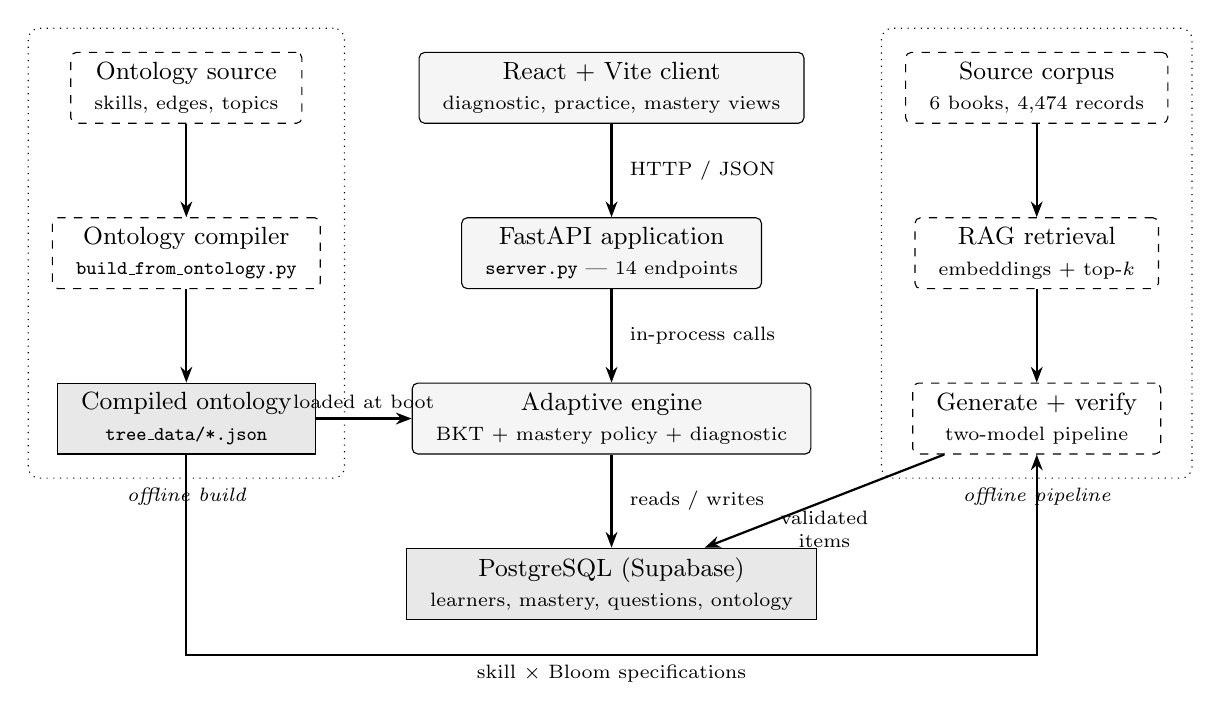
\begin{tikzpicture}[
      font=\small,
      box/.style={draw, rounded corners=2pt, align=center, minimum height=9mm,
                  inner xsep=3mm, fill=gray!8},
      store/.style={draw, align=center, minimum height=9mm, inner xsep=3mm,
                    fill=gray!18},
      off/.style={draw, dashed, rounded corners=2pt, align=center,
                  minimum height=9mm, inner xsep=3mm},
      arr/.style={-{Stealth[length=2mm]}, thick}
    ]
    % --- serving path -------------------------------------------------
    \node[box] (ui) at (0,0) {React + Vite client\\{\scriptsize diagnostic, practice, mastery views}};
    \node[box] (api) at (0,-2.1) {FastAPI application\\{\scriptsize \texttt{server.py} --- 14 endpoints}};
    \node[box] (engine) at (0,-4.2) {Adaptive engine\\{\scriptsize BKT $+$ mastery policy $+$ diagnostic}};
    \node[store] (db) at (0,-6.3) {PostgreSQL (Supabase)\\{\scriptsize learners, mastery, questions, ontology}};

    \draw[arr] (ui) -- node[right=1mm]{\scriptsize HTTP / JSON} (api);
    \draw[arr] (api) -- node[right=1mm]{\scriptsize in-process calls} (engine);
    \draw[arr] (engine) -- node[right=1mm]{\scriptsize reads / writes} (db);

    % --- ontology ------------------------------------------------------
    \node[store] (onto) at (-5.4,-4.2) {Compiled ontology\\{\scriptsize \texttt{tree\_data/*.json}}};
    \node[off] (build) at (-5.4,-2.1) {Ontology compiler\\{\scriptsize \texttt{build\_from\_ontology.py}}};
    \node[off] (src) at (-5.4,0) {Ontology source\\{\scriptsize skills, edges, topics}};
    \draw[arr] (src) -- (build);
    \draw[arr] (build) -- (onto);
    \draw[arr] (onto) -- node[above]{\scriptsize loaded at boot} (engine);

    % --- content pipeline ----------------------------------------------
    \node[off] (corpus) at (5.4,0) {Source corpus\\{\scriptsize 6 books, 4{,}474 records}};
    \node[off] (rag) at (5.4,-2.1) {RAG retrieval\\{\scriptsize embeddings $+$ top-$k$}};
    \node[off] (gen) at (5.4,-4.2) {Generate $+$ verify\\{\scriptsize two-model pipeline}};
    \draw[arr] (corpus) -- (rag);
    \draw[arr] (rag) -- (gen);
    \draw[arr] (gen) -- node[below, align=center]{\scriptsize validated\\[-1mm]\scriptsize items} (db);
    \draw[arr] (onto.south) |- (-5.4,-7.2) -- node[below]{\scriptsize skill $\times$ Bloom specifications} (5.4,-7.2) -| (gen.south);

    \begin{scope}[on background layer]
      \node[draw, dotted, rounded corners, fit=(src)(build)(onto), inner sep=3mm,
            label={[font=\scriptsize\itshape]below:offline build}] {};
      \node[draw, dotted, rounded corners, fit=(corpus)(rag)(gen), inner sep=3mm,
            label={[font=\scriptsize\itshape]below:offline pipeline}] {};
    \end{scope}
  \end{tikzpicture}
  \caption{System architecture. Solid boxes are the online serving path;
    dashed boxes are offline processes that run before serving and write their
    artefacts into the compiled ontology and the question bank.}
  \label{fig:architecture}
\end{figure}

\begin{table}[htbp]
  \centering
  \caption{Subsystem responsibilities}
  \label{tab:modules}
  \begin{tabularx}{\textwidth}{>{\hsize=0.55\hsize}Y>{\hsize=0.7\hsize}Y>{\hsize=1.75\hsize}Y}
    \toprule
    Subsystem & Location & Responsibility \\
    \midrule
    Knowledge ontology & \path{Ontology/}, \path{Backend/tree_data/} & Defines skills, their Bloom levels, their topics, and the prerequisite edges between them. Compiled from source into the served JSON artefacts by a build script that enforces acyclicity and applies transitive reduction. \\
    Inference engine & \path{Backend/bkt.py}, \path{bloom_taxonomy.py}, \path{mastery_updater.py}, \path{skill.py}, \path{skill_tree.py} & Maintains and updates per-skill mastery; owns the graph, its cycle check and its topological ordering. \\
    Session logic & \path{Backend/diagnostic.py}, session state in \path{server.py} & Runs a diagnostic or practice session: which skill to test next, which Bloom level, which question, when to stop. \\
    Serving API & \path{Backend/server.py} & Exposes catalogue, session and mastery endpoints; composes engine and database. \\
    Content pipeline & \path{data-gen/} & Parses the corpus, builds a retrieval index, generates and verifies questions, loads them to the database. \\
    Client & \path{Frontend/} & Renders the catalogue, question flow and mastery views; handles bilingual display and mathematical typesetting. \\
    \bottomrule
  \end{tabularx}
\end{table}

\paragraph{Where standards shaped the partition.} Two boundaries in
\Cref{fig:architecture} exist for reasons from \Cref{sec:standards} rather than
for reasons of convenience. First, the privileged database key lives only in the
API process: the client never holds a credential that can write to the database,
which is why there is no direct client-to-database arrow even though the
database vendor supports one. Second, the corpus sits strictly inside the
offline pipeline and is never served: generated items reach the database, but
the copyrighted source text never leaves the build environment.

\paragraph{Safety considerations.} The system carries no physical-safety risk,
but it does carry a decision-quality risk: a learner may reallocate study time
during a high-stakes year on the strength of a wrong inference. The design
response is conservatism in the gating policy --- the threshold for declaring a
prerequisite mastered is deliberately high (0.95), so the system prefers to keep
a learner practising a foundation slightly too long over releasing them from it
too early.

\section{Design Refinement and Simulation}
\label{sec:detailed-design}

\subsection{The knowledge-tracing model}
\label{sec:bkt-model}

Each skill's mastery is a latent binary variable; the engine maintains
$P(L_n)$, the probability that the learner has learned the skill after $n$
opportunities. Four parameters govern its evolution: the prior $P(L_0)$, the
learning rate $P(T)$, the slip probability $P(S)$ and the guess probability
$P(G)$ \cite{corbett1995knowledge}. Each response triggers a two-step update.

Step 1, the Bayesian posterior given the observed response:
\begin{align}
  P(L_n \mid \text{correct}) &=
    \frac{P(L_n)\,\bigl(1-P(S)\bigr)}
         {P(L_n)\,\bigl(1-P(S)\bigr) + \bigl(1-P(L_n)\bigr)\,P(G)}
  \label{eq:posterior-correct}\\[2mm]
  P(L_n \mid \text{incorrect}) &=
    \frac{P(L_n)\,P(S)}
         {P(L_n)\,P(S) + \bigl(1-P(L_n)\bigr)\,\bigl(1-P(G)\bigr)}
  \label{eq:posterior-incorrect}
\end{align}

Step 2, the learning transition --- the chance that the opportunity itself
taught the skill:
\begin{equation}
  P(L_{n+1}) = P(L_n \mid \text{evidence})
             + \bigl(1 - P(L_n \mid \text{evidence})\bigr)\,P(T)
  \label{eq:transition}
\end{equation}

Mastery is persisted as a percentage on $[0,100]$ and related to the
probability form by $P(L) = \text{mastery}/100$. The implementation is
deliberately \emph{stateless} --- it takes a probability and an observation and
returns a probability, holding no learner state --- so that the entire model can
be replaced by an individualised or neural variant
\cite{yudelson2013individualized,piech2015deep} without altering a single call
site. That is the concrete design provision for the successor identified in
\Cref{sec:alternatives}.

\subsection{Conditioning the noise parameters on cognitive level}

The refinement that distinguishes this engine from textbook BKT is that $P(G)$
and $P(S)$ are not constants but functions of the question's Bloom level. A
four-option recall item is guessable; an analysis item is not. Conversely, a
learner who knows an analysis-level procedure has more opportunities to slip
while executing it. \Cref{tab:bloom-params} gives the values used.

\begin{table}[htbp]
  \centering
  \caption{Bloom-conditioned guess and slip parameters, and the mastery band each level occupies}
  \label{tab:bloom-params}
  \begin{tabular}{lccc}
    \toprule
    Bloom level & $P(G)$ & $P(S)$ & Mastery band \\
    \midrule
    Remember   & 0.30 & 0.05 & 0.00 -- 16.67 \\
    Understand & 0.25 & 0.08 & 16.67 -- 33.33 \\
    Apply      & 0.18 & 0.12 & 33.33 -- 50.00 \\
    Analyze    & 0.12 & 0.18 & 50.00 -- 66.67 \\
    Evaluate   & 0.08 & 0.22 & 66.67 -- 83.33 \\
    Create     & 0.05 & 0.25 & 83.33 -- 100.00 \\
    \bottomrule
  \end{tabular}
\end{table}

The 0--100 mastery scale is partitioned into six equal bands of
$100/6 \approx 16.67$ points, one per level, so that a mastery value maps
directly to a cognitive level. This is what makes the selection rule expressible:
the next question is requested one band above the learner's current band, which
is the zone-of-proximal-development rule \cite{vygotsky1978mind} rendered
arithmetically.

\subsection{The three-phase mastery update policy}
\label{sec:mastery-policy}

Every response runs three phases in order.

\textbf{Phase 1 --- Bloom-conditioned BKT.} Look up $P(G), P(S)$ for the
question's Bloom level, compute the effective transition rate (Phase 3), and
apply \Cref{eq:posterior-correct,eq:posterior-incorrect,eq:transition} to the
answered skill.

\textbf{Phase 2 --- Ancestor pull-up.} If the response was correct, traverse the
skill's ancestors breadth-first and raise each to at least the answered skill's
new posterior:
\begin{equation}
  P(a) \leftarrow \max\bigl(P(a),\, P(s)\bigr)
  \qquad \forall a \in \operatorname{ancestors}(s)
  \label{eq:pullup}
\end{equation}
The justification is evidential: correctly executing a skill is evidence that
its prerequisites are held, because the skill is not executable without them.
The asymmetry is deliberate --- an \emph{incorrect} response propagates nothing
downward to prerequisites, because failure is ambiguous. It may indicate a
missing prerequisite, but it may equally indicate a slip at the top level, and
penalising every ancestor for one wrong answer would make the estimate
unstable. Locating the responsible prerequisite is instead the job of the
spillover rules, which use option-level evidence rather than a blanket penalty.

\textbf{Phase 3 --- Conjunctive transition gating.} A skill's learning rate is
not constant. For a skill $s$ with direct prerequisites
$\operatorname{parents}(s)$:
\begin{equation}
  P(T)_s =
  \begin{cases}
    \tau_{\text{base}} & \text{if } \min_{p \in \operatorname{parents}(s)} P(L_p) \ge \theta \\[1mm]
    \tau_{\text{locked}} & \text{otherwise}
  \end{cases}
  \label{eq:gating}
\end{equation}
with $\theta = 0.95$, $\tau_{\text{base}} = 0.10$ in normal practice,
$0.20$ during a diagnostic (where the aim is to move the estimate quickly), and
$\tau_{\text{locked}} = 0.01$. The gate is \emph{conjunctive} --- every
prerequisite must clear the threshold, not merely the average or the best one.
This is the formal expression of the project's central claim: a learner cannot
be credited with advancing on a skill while a foundation beneath it is missing.
Its correctness depends entirely on $\operatorname{parents}(s)$ being the
\emph{direct} prerequisites, which is why the ontology build applies transitive
reduction (\Cref{sec:ontology-rebuild}); a redundant shortcut edge would let a
skill unlock while its true intermediate prerequisite was still unmastered.

\subsection{Adaptive question selection}

A diagnostic of tractable length cannot test 1{,}688 skills --- a section's
worth is already far more than a learner will sit through --- so it must choose
skills whose outcome is maximally informative about the rest of the graph. The engine
scores each untested skill by a balanced-volume heuristic:
\begin{equation}
  \operatorname{score}(s) =
  \frac{u_{\uparrow}(s) + u_{\downarrow}(s) + 1}
       {1 + \lvert u_{\uparrow}(s) - u_{\downarrow}(s) \rvert}
  \label{eq:selection}
\end{equation}
where $u_{\uparrow}$ and $u_{\downarrow}$ are the counts of untested ancestors
and untested descendants. The numerator rewards skills that touch many unknowns;
the denominator rewards \emph{balance}. A skill with 20 unknown descendants and
no unknown ancestors is a root whose failure tells us little about what lies
above it; a skill sitting between two large unknown regions bisects the graph,
and its outcome constrains both directions. This is the knowledge-space insight
\cite{doignon1985spaces} applied as a greedy heuristic.

Priors are initialised by depth: root skills start at 0.70 mastery and the
deepest skills at 0.20, interpolated linearly between, encoding the assumption
that foundational material is more likely already held.

Having chosen a skill and a target Bloom level, the engine searches for an item
through a fallback ladder, because the ideal item frequently does not exist in
a partially generated bank: (i) same skill, nearby Bloom level, matching topic;
(ii) same skill, nearby Bloom level, any topic; (iii) same topic, graph-nearby
skills ordered by distance, preferring the lowest-mastery candidate. ``Nearby
Bloom'' means the offsets $[0,+1,-1,+2,-2,+3,-3]$ tried in that order. If no
tier yields an item, the skill is marked tested and the session advances --- the
design decision that a missing question must never stall a session (NFR3).

\subsection{Prerequisite spillover}

During topic practice, two rules detect that failure is caused by something
upstream rather than by the topic itself. Rule A fires when at least three of
the last five wrong answers implicate the same missing prerequisite, evidence
that comes from the \texttt{option\_missing\_prerequisites} table --- each
distractor is annotated with the skill whose absence would lead a learner to
choose it. Rule B fires when rolling accuracy over the last eight attempts falls
below 40\% \emph{and} some candidate prerequisite has mastery below 0.60; the
weakest such prerequisite is chosen. Either rule injects two prerequisite-focused
questions before returning to the topic traversal. Rule A is precise but needs
distractor annotations; Rule B is a coarser safety net that works without them.

\subsection{The skill graph, and its rebuild}
\label{sec:ontology-rebuild}

\begin{figure}[htbp]
  \centering
  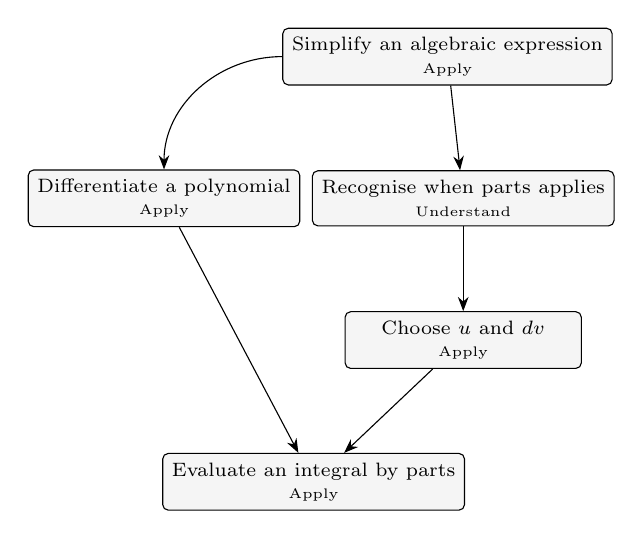
\begin{tikzpicture}[
      font=\scriptsize,
      skill/.style={draw, rounded corners=2pt, minimum width=30mm,
                    minimum height=7mm, align=center, fill=gray!8},
      arr/.style={-{Stealth[length=1.8mm]}}
    ]
    \node[skill] (alg)  at (0,0)    {Simplify an algebraic expression\\{\tiny Apply}};
    \node[skill] (diff) at (-3.6,-1.8) {Differentiate a polynomial\\{\tiny Apply}};
    \node[skill] (rec)  at (0.2,-1.8)  {Recognise when parts applies\\{\tiny Understand}};
    \node[skill] (pick) at (0.2,-3.6)  {Choose $u$ and $dv$\\{\tiny Apply}};
    \node[skill] (ibp)  at (-1.7,-5.4) {Evaluate an integral by parts\\{\tiny Apply}};

    \draw[arr] (alg) -- (rec);
    \draw[arr] (rec) -- (pick);
    \draw[arr] (pick) -- (ibp);
    \draw[arr] (diff) -- (ibp);
    \draw[arr] (alg) to[out=180,in=90] (diff);
  \end{tikzpicture}
  \caption{A fragment of the skill graph, illustrating the granularity target.
    ``Integration by parts'' is not one node but a chain: recognising
    applicability, choosing the decomposition, and executing it --- each
    separately testable, and each with its own prerequisites, so that a failure
    can be localised to the step that actually broke.}
  \label{fig:skill-fragment}
\end{figure}

The first ontology was derived from a sample of the corpus and yielded 430
skills across 66 topics with 471 edges. In use it proved too coarse: a topic
held on average fewer than four skills, so a failure inside a topic could not be
localised further, and the conjunctive gate had too few edges to act on. The
graph was therefore rebuilt from the complete corpus --- all 4{,}474 parsed
records of all six books --- at a granularity where a node names one action, and
the rebuild is now the catalogue the application serves.
\Cref{tab:ontology-compare} compares the two. The two edge counts given there
are both real and differ for a reason worth stating: the ontology source asserts
1{,}743 prerequisite relations, and the build's transitive reduction removes the
60 that are implied by a longer path, leaving 1{,}683 direct edges in the
compiled catalogue. It is the compiled figure that \Cref{eq:gating} acts on.

\begin{table}[htbp]
  \centering
  \caption{Legacy ontology versus full-corpus rebuild}
  \label{tab:ontology-compare}
  \begin{tabular}{lrr}
    \toprule
    Property & Legacy (superseded) & Rebuild (served) \\
    \midrule
    Skills & 430 & 1{,}688 \\
    Prerequisite edges (source) & 471 & 1{,}743 \\
    Prerequisite edges (compiled) & 471 & 1{,}683 \\
    Topics covered & 66 & 183 of 183 \\
    Corpus coverage & sample & all 4{,}474 records \\
    Maximum graph depth & 7 & 9 \\
    Isolated skills & --- & 0 \\
    Unresolved prerequisite references & --- & 0 \\
    Connected components (largest) & --- & 87 (482) \\
    \bottomrule
  \end{tabular}
\end{table}

\begin{table}[htbp]
  \centering
  \caption{Rebuilt ontology by subject}
  \label{tab:ontology-subject}
  \begin{tabular}{lrrrr}
    \toprule
    Subject & Skills & Edges & Edges per skill & Topics \\
    \midrule
    Chemistry   & 886 & 868 & 0.97 & 59 \\
    Mathematics & 446 & 499 & 1.10 & 52 \\
    Physics     & 356 & 376 & 1.06 & 72 \\
    \midrule
    Total       & 1{,}688 & 1{,}743 & 1.03 & 183 \\
    \bottomrule
  \end{tabular}
\end{table}

The build is reproducible rather than hand-maintained: a compiler reads the
ontology source, applies an editorial layer (topic aliases and display labels),
checks the graph for cycles, applies transitive reduction, and emits the JSON
artefacts the server loads. Transitive reduction is not cosmetic --- as
\Cref{eq:gating} shows, a shortcut edge would let a skill unlock while its true
intermediate prerequisite was unmastered.

\subsection{Data model}

\begin{table}[htbp]
  \centering
  \caption{Database schema}
  \label{tab:schema}
  \begin{tabularx}{\textwidth}{>{\hsize=0.65\hsize}Y>{\hsize=1.35\hsize}Y}
    \toprule
    Table & Contents and constraints \\
    \midrule
    \texttt{users} & Learner identity: surrogate UUID, unique username. \\
    \texttt{user\_skill} & Per-learner, per-skill mastery on $[0,100]$; composite primary key; cascades on learner or skill deletion. \\
    \texttt{skills} & Skill identifier and description; description is NOT NULL. \\
    \texttt{questions} & Stem, Bloom level, and topic. \texttt{topic} is a foreign key to \texttt{ontology\_topics}, so it stores a topic \emph{code}, never a display label. \\
    \texttt{question\_options} & Four options per question, label constrained to A--D, correctness flag, and a per-option explanation. \\
    \path{option_missing_prerequisites} & Maps a distractor to the skill whose absence explains choosing it --- the evidence source for spillover Rule A. \\
    \texttt{ontology\_topics}, \texttt{ontology\_skill\_topics}, \texttt{ontology\_skill\_edges} & The ontology mirrored into the database for referential integrity of questions and skills. \\
    \bottomrule
  \end{tabularx}
\end{table}

Two deliberate omissions are worth stating. There is no \texttt{subject} column
anywhere: subject is a property of the ontology, derived at read time and
plumbed through the API, so that the database never holds a second copy of a
fact the ontology owns. And the transition probability $P(T)_s$ is not
persisted: it is recomputed from current parent mastery on every request, so it
can never fall out of sync with the values it is derived from.

\subsection{API surface}

The API is a flat, session-oriented REST surface of 14 endpoints
(\Cref{tab:api}). The two session families are deliberately symmetric ---
\texttt{start}, \texttt{status}, \texttt{next}, \texttt{answer} --- so the client
can drive either flow with one component.

\begin{table}[htbp]
  \centering
  \caption{API endpoints}
  \label{tab:api}
  \begin{tabularx}{\textwidth}{>{\hsize=1.05\hsize}Y>{\hsize=0.95\hsize}Y}
    \toprule
    Endpoint & Purpose \\
    \midrule
    \texttt{GET /catalog} & Courses, sections and topics from the compiled ontology \\
    \texttt{GET /users/\{name\}/}, \texttt{POST /users/} & Look up and create a learner \\
    \texttt{GET .../sections/\{id\}/state} & Diagnostic gate and lock state for a section \\
    \texttt{GET .../sections/\{id\}/mastery} & Mastery graph and table for visualisation \\
    \texttt{POST .../diagnostic/retake} & Reset section mastery and clear its sessions \\
    \texttt{POST /diagnostic/start} & Begin a diagnostic session \\
    \texttt{GET /diagnostic/\{id\}/status}, \texttt{/next} & Session progress; fetch next selected question \\
    \texttt{POST /diagnostic/\{id\}/answer} & Submit a response; triggers the three-phase update \\
    \texttt{POST /topic-practice/start} & Begin practice on one topic \\
    \texttt{GET /topic-practice/\{id\}/status}, \texttt{/next} & Progress; next question, including injected spillover items \\
    \texttt{POST /topic-practice/\{id\}/answer} & Submit a response; evaluates spillover rules \\
    \bottomrule
  \end{tabularx}
\end{table}

\subsection{Content generation pipeline}
\label{sec:generation-pipeline}

The pipeline turns the corpus into items aligned to the ontology. Source books
are parsed into structured records; a multilingual embedding model
\cite{reimers2019sentence} indexes them; for each (skill, Bloom level)
specification the top-$k$ relevant records are retrieved and supplied to a
generator model as grounding \cite{lewis2020retrieval}.

The design decision that matters most is the second stage. A generated item is
not accepted on the generator's own word: a \emph{different, cheaper} model
independently checks that the item is on-topic for the claimed skill, and
\emph{blind re-solves} it --- it is shown the question and options but not the
marked answer --- and the item is accepted only if its independent answer agrees
with the marked one. Letting a model grade its own output biases towards false
confidence; an independent judge with no sight of the expected answer is a real
check. The cost asymmetry is deliberate: generation uses the stronger model
because it is the harder task, verification uses the cheaper one because
agreement checking is easier than authoring, and verification calls are batched
across several specifications to reduce call count.

\subsection{Design calculations}

\textbf{Generation space.} With one item per (skill, Bloom level) pair, the
legacy ontology implies $430 \times 6 = 2{,}580$ specifications; the rebuilt
ontology implies $1{,}688 \times 6 = 10{,}128$. At the observed generation
pattern this is the dominant cost driver in the project and the reason adoption
of the rebuilt ontology is gated on a budgeted generation run
(\Cref{sec:budget}).

\textbf{Storage.} A question with four options and explanations occupies on the
order of a few kilobytes. A complete bank at rebuild scale is therefore of the
order of tens of megabytes --- immaterial against any database tier. Learner
data is smaller still: one row per learner per skill, so a cohort of
$10{,}000$ learners against 1{,}688 skills is under $2\times10^7$ rows of two
identifiers and a float, which is well within commodity capacity.

\textbf{Inference cost.} One response costs one constant-time Bayesian update
plus an ancestor traversal bounded by graph depth (9) and a successor refresh
over direct children. The engine is not the scaling bottleneck; database round
trips during question search are.

\section{Application of Tools}
\label{sec:tools}

% Rendered as a longtable (not a float) so it flows across pages at readable
% size instead of being squeezed onto one rotated page.
\setlength{\LTcapwidth}{\textwidth}
{\small\setstretch{1.1}
\begin{longtable}{@{}p{30mm}p{52mm}p{\dimexpr\textwidth-30mm-52mm-4\tabcolsep\relax}@{}}
  \caption{Tool selection, justification, and relevant limitations}
  \label{tab:tools}\\
    \toprule
    Tool & Why selected & Relevant limitations \\
    \midrule
  \endfirsthead
    \multicolumn{3}{@{}l}{\small\itshape \tablename~\thetable{} --- continued from previous page}\\[2pt]
    \toprule
    Tool & Why selected & Relevant limitations \\
    \midrule
  \endhead
    \midrule
    \multicolumn{3}{r@{}}{\small\itshape continued on next page}\\
  \endfoot
    \bottomrule
  \endlastfoot
    Python 3 & The engine is mathematical and graph-oriented; Python keeps \Cref{eq:posterior-correct}--\Cref{eq:gating} readable enough to audit against the policy document. & Slower than a compiled language --- immaterial here, since the update is constant-time. \\
    FastAPI $+$ Uvicorn & Typed request/response models via Pydantic catch malformed payloads at the boundary; automatic OpenAPI documentation made the API self-describing for the frontend developers. & The asynchronous model gives no benefit as used, since the engine is synchronous and CPU-light. \\
    Supabase (PostgreSQL) & A managed relational store with a usable free tier. Relational integrity is not optional here --- foreign keys are what stop a question referencing a skill that no longer exists. & The free tier pauses idle projects; the client library adds a network round trip where raw SQL would allow one query. \\
    React 18 $+$ Vite & Component model suits a question-at-a-time flow with shared state; Vite's fast rebuilds mattered on laptop hardware. & Single-page delivery means a large first-load bundle, worsened by mathematical typesetting fonts. \\
    KaTeX & Renders \LaTeX{} mathematics synchronously and quickly, and outputs accessible markup rather than images \cite{wcag21}. & Supports a subset of \LaTeX{}; unsupported macros in generated content must be caught before serving. \\
    Tailwind CSS & Utility classes kept styling consistent across developers without a design system. & Verbose markup; class strings are hard to review in diffs. \\
    Gemini API & After local generation proved infeasible on CPU (\Cref{sec:feasibility}), a hosted model supplied the throughput; free-tier keys could be pooled to raise it further. & Rate limits shape the pipeline's architecture; a hosted model is a dependency the project does not control, and model updates can silently change output quality. \\
    Sentence-transformers & Multilingual embeddings are required for a Bangla corpus; English-only models retrieve poorly here \cite{reimers2019sentence}. & A large download and CPU-bound indexing; embedding quality on Bangla mathematical text is materially worse than on English prose. \\
    Git and GitHub & Version control and the integration point for five developers working on separable subsystems. & --- \\
\end{longtable}}

\section{Implementation}
\label{sec:implementation}

\textbf{Engine.} The model was implemented from the equations rather than from a
library, which was the right call for auditability: the policy document and the
code state the same constants, and a reviewer can check one against the other.
The graph enforces its own invariant --- adding a prerequisite edge provisionally
inserts it, runs a three-colour depth-first search over the whole graph, and
rolls the edge back if it would close a cycle. The graph cannot enter an invalid
state through the public interface.

\textbf{Ontology.} Generated artefacts are never hand-edited. The source is
compiled by script, and the editorial decisions that cannot be derived from data
--- topic aliases, display labels, course and section layout --- live in a single
configuration file. Rebuilding is a one-command operation, which is what made a
late full rebuild affordable.

\textbf{Content pipeline.} Two failures shaped the implementation more than any
design intent. The first: source books are machine-extracted, and one corrupt
record in the Chemistry corpus --- a string containing a \LaTeX{} macro repeated
tens of thousands of times and never terminated --- desynchronised the parser and
destroyed 334 neighbouring records. The parser was rewritten to resynchronise
by decoding one object at a time, so a bad record now costs only itself. The
second: language models emit \LaTeX{} with single backslashes, and a strict JSON
parser silently consumes several of those escapes as control characters rather
than raising an error, corrupting text invisibly. This affected a measured
13.4\% of one early batch. The fix is an escape-repair pass applied before every
parse, in both the ingest and generation paths. Both failures are documented in
the repository so that a future contributor does not rediscover them.

\textbf{Frontend.} The mathematics rendering component is the non-obvious piece:
it splits mixed Bangla-and-\LaTeX{} strings on delimiters, renders the
mathematical segments through KaTeX, renders the rest as text, and normalises
newline sequences that arrive literally from generated content.

\textbf{Process.} Work was carried out in a shared Git repository with
subsystem-aligned branches merged into a main line --- 93 commits across roughly
five and a half months from five contributors. In place of a formal CI service,
the project relies on a credential-free test harness that any developer can run
in seconds before merging (\Cref{sec:evaluation}), plus a chain of handover
documents that record the state and rationale of each subsystem at the point it
changed hands. Those documents are themselves an engineering artefact: they
exist because the project spanned several months and five people, and knowledge
that lived only in one contributor's head was repeatedly found to be the
project's real bottleneck.

\section{Deployment}
\label{sec:deployment}

\textbf{Target environment.} The system deploys as two processes and one managed
service: a Python ASGI application serving the API, a static bundle for the
client, and the hosted PostgreSQL instance. A container definition is provided
for the backend. Configuration is by environment variables --- the database URL
and service key --- supplied through a file that is excluded from version
control; the client takes the API base URL at build time and defaults to the
local backend.

\textbf{Release process.} The ontology is compiled and its report inspected;
generated questions are validated and loaded with a dry run first; the backend
and client are then started. The deliberate ordering reflects the dependency
chain in \Cref{fig:architecture}: content cannot be loaded against an ontology
that has not been compiled.

\textbf{Operation and maintenance.} The prototype is operated by the project
team. Monitoring is limited to structured logging of question-search behaviour
--- each search prints which tier matched and how long the database query took,
which is what made the topic-code defect in \Cref{sec:revisions} visible.
Backup is delegated to the managed database service.

\textbf{Resources consumed.} One small application process (well under a
gigabyte of memory, since the loaded graph is a few thousand nodes), one static
file bundle, and a database holding tens of megabytes. Offline, the pipeline
consumes CPU for embedding the corpus and external API calls for generation ---
the only materially resource-hungry part of the system, and the subject of the
environmental assessment in \Cref{sec:sustainability}.

% Chapter 5 -- Rubric: PO4 (4.1)
\chapter{Investigation and Evaluation}
\label{ch:evaluation}

\section{Experimental Investigation}
\label{sec:investigation}

This is a development-focused project, so the investigations reported here are
those that validated --- or refuted --- specific design decisions. Four are
presented. Each states the question it was asked to settle, the method, and the
conclusion actually drawn, including the two cases where the investigation
overturned the team's initial position.

\subsection{Investigation 1: is local model inference viable for content generation?}

\textbf{Question.} Can the question bank be generated on the team's own hardware
using locally hosted open-weight models, avoiding any external API dependency
and any cost?

\textbf{Method.} A generation pipeline was implemented against locally served
quantised models (7B and 3B parameter classes) on CPU-only laptops, and measured
on real specifications drawn from the ontology, with prompt sizes of roughly
4--6\,k tokens and completions of roughly 3\,k tokens per call.

\textbf{Findings.} Two independent failures. On throughput, the measured
per-call latency extrapolated to multiple weeks of continuous computation for a
single full pass over the 2{,}580-specification space then in scope --- longer
than the remaining project schedule, on machines also needed for development. On
correctness, a subtler defect appeared: models emit \LaTeX{} commands such as
\verb|\tan| and \verb|\frac| with single backslashes, and a strict JSON parser
does not reject these --- for the subset of letters that happen to be legal JSON
escapes it silently consumes the backslash and substitutes a control character.
The corruption therefore produced no error at all, and was found only by reading
output.

\textbf{Conclusion.} The local approach was abandoned on throughput grounds, and
a hosted API adopted with key pooling to raise the rate ceiling. The escape
defect was not specific to local models --- it recurred with the hosted model at a
measured 13.4\% of one early production batch --- so an escape-repair pass was
made unconditional in both the ingest and generation paths. This is the clearest
case in the project of an investigation changing the architecture: the design in
\Cref{sec:generation-pipeline} exists because this one failed.

\subsection{Investigation 2: is the ontology's granularity sufficient to support the gating policy?}

\textbf{Question.} The conjunctive gate in \Cref{eq:gating} acts on a skill's
direct prerequisites. Does the first ontology supply enough structure for that
gate to do anything?

\textbf{Method.} Structural analysis of the 430-skill graph: skills per topic,
syllabus coverage, and the fraction of skills with no prerequisite edge at all.

\textbf{Findings.} Two deficits, both fatal to the gate. The graph averaged
fewer than four skills per topic, and a topic holding three skills cannot
localise a failure \emph{within} itself --- which is the system's entire
purpose. And a substantial fraction of skills had no incoming edge at all; a
gate with no parents to test degenerates to the ungated case, so for those
skills \Cref{eq:gating} was doing nothing.

Note that the binding measure here is coverage and connectedness, not the raw
edges-per-skill ratio. That ratio is similar before and after the rebuild
(1.1 against 1.03), and deliberately so: the rebuild added roughly four times
as many skills, so holding the ratio while eliminating isolated skills entirely
means the edges are distributed across the graph rather than concentrated in a
few dense topics. A higher ratio achieved by piling edges onto already-connected
skills would not have fixed either deficit above.

\textbf{Conclusion.} The ontology, not the engine, was the binding constraint.
This motivated the full-corpus rebuild (\Cref{sec:ontology-rebuild}), which
raised the graph to 1{,}688 skills and 1{,}743 edges with every one of the 183
syllabus topics populated and no isolated skills. \Cref{tab:ontology-effects}
reports the rebuild's structural effect.

\begin{table}[htbp]
  \centering
  \caption{Structural effect of the ontology rebuild and its editorial pass}
  \label{tab:ontology-effects}
  \begin{tabular}{lrr}
    \toprule
    Property & Before editorial pass & After \\
    \midrule
    Syllabus topics holding no skill & 54 & 0 \\
    Unresolved prerequisite references & 46 & 0 \\
    Isolated skills (no edge at all) & 6 & 0 \\
    Topics with no internal learning order & 5 & 0 \\
    Near-orphan fragments (2--6 skills) & 91 & 32 \\
    Connected components & 187 & 87 \\
    Largest connected component & 203 & 482 \\
    Maximum DAG depth & 7 & 9 \\
    \bottomrule
  \end{tabular}
\end{table}

\subsection{Investigation 3: can prerequisite edges be proposed mechanically?}

\textbf{Question.} After the rebuild, 91 fragments of 2--6 skills remained
disconnected from the main graph. Can the missing edges be proposed
automatically rather than authored by hand?

\textbf{Method.} Two scoring functions were implemented and their proposals
read individually against the subject matter. The first scored candidate parents
by token overlap with the orphaned skill. The second scored by
\emph{topic hub-ness} --- preferring the candidate at the lowest Bloom tier with
the most dependents.

\textbf{Findings.} Token overlap produced roughly 40\% usable proposals. Its
failures were systematic rather than random: it proposed lateral links between
peers that merely share vocabulary --- zero-order kinetics ``requiring''
first-order kinetics, the cosine rule ``requiring'' the sine rule --- and in one
case proposed a pair in both directions, which would have closed a cycle.
Hub-based scoring raised usable proposals to roughly two thirds. Of 83 proposals
finally reviewed, 48 were applied (several with the direction reversed from what
was proposed) and 35 were rejected outright, their fragments left deliberately
disconnected rather than wrongly connected.

\textbf{Conclusion.} Mechanical proposal is a useful accelerator and an
unacceptable authority. A wrong prerequisite edge is worse than a missing one,
because \Cref{eq:pullup} propagates along it and will credit a learner for a
skill they have never demonstrated. The 32 fragments that survive are recorded
as requiring a domain expert rather than another heuristic.

\subsection{Investigation 4: do automated quality heuristics over-flag?}

\textbf{Question.} Two validators were written to find defects in the generated
ontology: one flagging skills that fuse two actions, and one flagging ``Bloom
inversions'' --- edges whose prerequisite sits at a \emph{higher} Bloom tier than
the skill requiring it. Are their outputs trustworthy?

\textbf{Method.} Every flag from both checks was read against the underlying
skill or edge.

\textbf{Findings.} The multi-action check flagged 173 skills, of which over half
were false positives, and was replaced by a stricter criterion yielding 47
candidates --- of which 20 were genuine splits and 27 were rejected on reading.
The Bloom-inversion check flagged 147 edges; hand review found \emph{3}
genuinely reversed. The check's premise was wrong, not the data: Bloom tier
measures cognitive demand, not teaching order, and a low-tier fact \emph{about}
an operation is routinely learned after the operation itself. For example,
recalling that a determinant with two equal rows is zero (Remember) legitimately
depends on being able to evaluate a determinant (Apply).

\textbf{Conclusion.} The inversion check was downgraded from error to advisory
rather than deleted, with its reasoning recorded so the next contributor does not
reinstate it. The transferable finding is that on this project mechanical
heuristics over-flagged by roughly the same large factor twice, and that the
correct response is to calibrate a heuristic against hand review before treating
its output as a defect list.

\section{Performance Evaluation}
\label{sec:evaluation}

\subsection{Setup and acceptance criteria}

The engine is evaluated by an automated end-to-end harness that runs the real
diagnostic, mastery-update, topic-practice and spillover code paths against an
in-memory stand-in for the database, seeded with a synthetic learner and a
question bank drawn from the compiled ontology. It requires no credentials and
no network, which is what makes it runnable by any developer before a merge.
Acceptance is binary per check: all checks must pass.

\subsection{Results}

The harness reports \textbf{18 checks passed, 0 failed}, reproduced on the
current tree against the adopted 1{,}688-skill ontology. \Cref{tab:smoke} lists
what each check establishes.

One property of the harness should be read before its results are interpreted.
It selects a section automatically and sizes the diagnostic to that section's
skill count, so the absolute figures it prints depend on which section it picks
--- on the current tree that is a small one (eight skills). The checks therefore
establish that each mechanism \emph{runs and holds its invariants}; they are not
a measurement of how far evidence propagates in a large section, which would
require a section with real depth and a populated question bank. The propagation
guarantee is carried by the invariant check, not by counting how many skills
moved.

\begin{table}[htbp]
  \centering
  \caption{End-to-end verification harness: checks and what each establishes}
  \label{tab:smoke}
  \begin{tabularx}{\textwidth}{>{\hsize=0.42\hsize}Y>{\hsize=0.82\hsize}Y>{\hsize=1.76\hsize}Y}
    \toprule
    Area & Check & Establishes \\
    \midrule
    Ontology & Graph builds (1{,}688 skills); catalogue topics all resolve (183); no legacy topic codes remain & The served ontology is internally consistent and the catalogue cannot reference a topic that does not exist \\
    Question search & Tier-1 filter matches by topic \emph{code}; filtering by display label matches nothing & Regression guard for the defect in \Cref{sec:revisions} \\
    Diagnostic & Session starts, sized to the section (8 skills in the section exercised); question carries its subject; topic shown as label (\texttt{PHY1\_ERRORS} $\rightarrow$ ``Errors and Significant Figures''); every question answered & The adaptive loop runs to completion, sizes itself to the section, and returns learner-presentable metadata (FR3, FR12) \\
    Mastery & Mastery unlocked after diagnostic; written to \texttt{user\_skill}; section state reports subject & The update path persists per-skill mastery and releases the diagnostic gate (FR4, FR7) \\
    Invariant & No ancestor sits below its descendant & \Cref{eq:pullup} holds globally after a full session --- the correctness property in NFR1 \\
    Mastery view & View unlocked; graph returns nodes and edges for the section; table rows carry subject & The visualisation contract holds (FR10) \\
    Practice & Topic practice serves and accepts questions & Post-diagnostic flow works (FR8) \\
    Spillover & Fires on repeated wrong answers, reporting its triggering rule (rule A, repeated missing prerequisite) & The prerequisite-detection policy triggers on the intended evidence (FR9) \\
    \bottomrule
  \end{tabularx}
\end{table}

The ontology is separately validated by a structural checker, which reports
\textbf{zero errors}: the graph is acyclic, every one of the 183 topics holds at
least one skill, no skill is isolated, and no prerequisite reference is
unresolved.

\subsection{Evaluation against requirements}

\Cref{tab:traceability} traces every functional and non-functional requirement
from \Cref{ch:requirements} to the evidence that it is met, or to the deviation
recorded in \Cref{sec:revisions} where it is not. Two entries are not claims of
success: FR13 is partially met and NFR2 was never measured.

\begin{table}[htbp]
  \centering
  \caption{Requirements traceability and status}
  \label{tab:traceability}
  \begin{tabularx}{\textwidth}{>{\hsize=0.3\hsize}Y>{\hsize=0.45\hsize}Y>{\hsize=2.25\hsize}Y}
    \toprule
    Req. & Status & Evidence or deviation \\
    \midrule
    FR1 & Met, reduced & Account creation and sign-in work, but without a password (\Cref{sec:deviations-auth}) \\
    FR2 & Met & Catalogue endpoint serves ontology-derived courses, sections and topics; verified by harness \\
    FR3 & Met & Diagnostic runs to a full 30-question session in the harness \\
    FR4 & Met & Bloom-conditioned update implemented per \Cref{tab:bloom-params}; exercised on every answered question \\
    FR5 & Met & Ancestor pull-up implemented; the invariant that no ancestor sits below its descendant is verified explicitly after a full session \\
    FR6 & Met & Conjunctive gate implemented per \Cref{eq:gating} \\
    FR7 & Met & Mastery view locked before, unlocked after the diagnostic \\
    FR8 & Met & Topic practice served and answered questions in the harness \\
    FR9 & Met & Spillover fired and reported its triggering rule \\
    FR10 & Met & Mastery graph (nodes and edges for the section) and table both returned \\
    FR11 & Met & Retake endpoint resets section mastery and clears sessions \\
    FR12 & Met & Mathematics renders through KaTeX; literal newline handling fixed during implementation \\
    FR13 & \textbf{Partially met} & Pipeline is complete and validated, but the bank covers only part of the specification space (\Cref{sec:eval-limits}) \\
    FR14 & Met & Interface strings available in English and Bangla \\
    \midrule
    NFR1 & Met & Acyclicity enforced at insertion; ancestor invariant checked by harness; validator reports zero errors \\
    NFR2 & \textbf{Not measured} & No latency benchmark was run (\Cref{sec:eval-limits}) \\
    NFR3 & Met & Fallback ladder exercised; a missing item marks the skill tested and advances \\
    NFR4 & Met & Ontology compiled from source by script; generated files are not hand-edited \\
    NFR5 & Met & Harness runs with no credentials and no network \\
    NFR6 & Met & Entire system developed and run on CPU-only laptops \\
    NFR7 & Met & Bangla content with \LaTeX{} mathematics end to end \\
    NFR8 & Met & Credentials held in a git-ignored environment file, server-side only \\
    \bottomrule
  \end{tabularx}
\end{table}

\subsection{Evaluation against objectives}

O1--O5, O7 and O8 are met as evidenced above.

\textbf{O6 (question bank) is partially met}, and the shortfall is worth
quantifying rather than leaving as an adjective. The pipeline is built,
validated, and has generated and loaded real verified items; what is incomplete
is coverage of the specification space. Two figures bound the gap. Against the
legacy 430-skill ontology the space was $430 \times 6 = 2{,}580$
(skill, Bloom level) specifications, and generation had reached roughly a fifth
of it when the rebuild superseded that target. Against the now-adopted
1{,}688-skill ontology the space is $1{,}688 \times 6 = 10{,}128$
specifications, and because the existing items are keyed to legacy skill
identifiers they do not transfer: coverage against the served ontology therefore
starts close to zero and the generation run is outstanding in full. This is the
same debt identified in \Cref{sec:deviations-adoption}, and it is the single
largest piece of remaining work (\Cref{sec:future}).

\textbf{O3 is met in implementation but unvalidated in effect} --- the
propagation is provably consistent, but whether the resulting estimates
correspond to real learner knowledge is exactly the question the next subsection
says was not answered.

\subsection{Limitations of this evaluation}
\label{sec:eval-limits}

The evaluation above is structural and functional. It establishes that the
system computes what it was designed to compute and that its invariants hold. It
does \textbf{not} establish that the system helps anyone learn, and the report
makes no such claim. Specifically:

\begin{itemize}
  \item \textbf{No human participants.} There was no user study, no classroom
    trial, and no usability testing with members of the target cohort. Every
    claim about learner benefit in this report is an argument from design, not a
    measurement.
  \item \textbf{No fitted parameters.} $P(L_0)$, $P(T)$ and the Bloom-conditioned
    $P(G), P(S)$ values are pedagogical priors, not estimates. The literature is
    explicit that fitted and individualised parameters outperform fixed ones
    \cite{yudelson2013individualized,baker2008more}; this system cannot do that
    until it has response data, which it cannot have before deployment.
  \item \textbf{No predictive validation.} The standard quantitative check on a
    knowledge-tracing model --- does it predict the next response better than a
    baseline, measured by AUC on held-out data --- was not performed, because
    there is no held-out learner data.
  \item \textbf{No performance benchmark.} NFR2 was not measured; the system is
    subjectively responsive in use, which is not evidence.
  \item \textbf{Ontology unreviewed by domain experts.} The rebuilt graph is
    structurally valid but its subject-matter correctness has been verified only
    by the team. 32 disconnected fragments and a body of hand-authored
    prerequisite edges are explicitly awaiting review by a chemist and a
    physicist.
  \item \textbf{Question bank coverage is partial}, so a full-coverage session is
    not yet reachable for every topic. Two consequences follow that the harness
    cannot surface, because it seeds synthetic items rather than reading the real
    bank. First, the Bloom ladder degrades: the engine requests a question one
    band above the learner's current band, and where the bank holds no item at
    that level the nearby-Bloom fallback
    ($[0,+1,-1,+2,-2,+3,-3]$) supplies whatever exists, so the cognitive
    progression the design intends is weaker in practice than in specification.
    Second, the graph-nearby search tiers are exercised far less than the
    fallback, for the same reason. Both resolve with coverage, not with code.
  \item \textbf{The harness measures mechanism, not magnitude.} It sizes each
    run to the section it selects, so its printed figures vary with that choice
    and are evidence that each path executes and its invariants hold --- not a
    measurement of how far evidence propagates across a large, well-connected
    section.
\end{itemize}

\section{Deviations and Design Revisions}
\label{sec:revisions}

\subsection{Topic filter matched no rows (found, analysed, fixed)}

\textbf{Deviation.} The diagnostic's first two search tiers returned nothing,
ever. Every question was silently arriving from the untargeted fallback, so
topic-targeted and graph-nearby selection --- two thirds of the selection design
--- were dead code in practice.

\textbf{Cause.} The \texttt{questions.topic} column is a foreign key to
\texttt{ontology\_topics} and therefore holds a topic \emph{code}
(\texttt{MAT\_MATRIX}), while the search filtered it by the catalogue
\emph{display label} (``Matrices and Determinants''). The two can never be
equal, so the filter matched no row. Nothing failed loudly: a query returning
zero rows is a valid query, and the fallback dutifully supplied a question, so
sessions looked healthy.

\textbf{Revision.} The filter was corrected to compare codes, and --- more
importantly --- two checks were added to the harness: one asserting that a
code-based filter matches, and one asserting that a label-based filter matches
\emph{nothing}. The second check is the one that matters; it fails if anyone
reintroduces the confusion.

\subsection{Session state is not persistent}
\label{sec:deviations-session}

\textbf{Deviation.} Diagnostic and practice sessions live in process memory, so
a backend restart discards every in-flight session (NFR-adjacent, and a
production defect).

\textbf{Analysis.} The session objects hold graph traversal state that was not
designed for serialisation. Persisting them properly means either a session
store or reconstructing session state from the durable mastery table on demand.

\textbf{Decision.} Not revised, deliberately. The deployment target for this
project is a single demonstration process where the failure mode is a lost
session rather than lost mastery --- mastery itself \emph{is} persisted. The
correct fix is recorded as production hardening rather than disguised.

\subsection{Authentication is username-only}
\label{sec:deviations-auth}

\textbf{Deviation.} A learner signs in with a username and no password; the
client holds the resulting identity in browser storage. This does not meet the
access-control expectations of \Cref{sec:standards}.

\textbf{Analysis.} The system stores no data that is sensitive in itself beyond
performance history, and the prototype's users are the team. Authentication was
therefore deprioritised against the ontology work, which was on the critical
path for every other subsystem.

\textbf{Decision.} Not revised within the project. It is the first item of
production hardening (\Cref{sec:future}), and is stated here rather than
presented as a design choice, because it is not one --- it is an accepted debt.

\subsection{Ontology adoption, and the coverage debt it exposes}
\label{sec:deviations-adoption}

\textbf{Deviation.} For most of the project the application served the 430-skill
legacy ontology while the validated 1{,}688-skill rebuild sat beside it,
unadopted. Adoption has since been carried out: the compiled catalogue in
\texttt{Backend/tree\_data/} is now generated from the rebuild --- 1{,}688
skills across all 183 syllabus topics --- and the generation pipeline's ontology
source has been repointed to the rebuild so that the two cannot drift apart.

\textbf{Analysis.} Adoption was deliberately held back rather than forgotten,
because it is not merely a file swap. The existing question bank is keyed to
legacy skill identifiers, so switching the catalogue does not carry the content
across with it: a system that knows about 1{,}688 skills but holds questions for
a fraction of them can diagnose more finely in principle while being able to ask
about less in practice. Adopting therefore converts a \emph{structural} deficit
into a \emph{coverage} deficit --- the right trade, because coverage is bought
by a generation run whereas structure had to be rebuilt by hand, but it is a
debt and is recorded as one.

\textbf{Decision.} Adopt, then generate --- the order finally taken, with the
consequence stated explicitly rather than presented as complete. The outstanding
generation run against the enlarged specification space is quantified in
\Cref{sec:budget} and carried as the first item of
\Cref{sec:future}. Until it is complete, question-bank coverage against the
served ontology is the system's binding limitation, and \Cref{sec:eval-limits}
records it as such.

% Chapter 6 -- Rubric: PO11, PO9 (9.1--9.4), PO6 (6.1), PO7 (7.1), PO8 (8.1--8.4)
\chapter{Project Management, Teamwork, and Impact}
\label{ch:management}

\section{Project Management and Finance}

\subsection{Planning and Risk Management}
\label{sec:plan}

The project ran across one academic session with five contributors, all carrying
a full course load. Work was partitioned along the subsystem boundaries of
\Cref{fig:architecture}, which was chosen partly for architectural reasons and
partly because those boundaries are the ones that let several people work
without blocking each other: the engine, the content pipeline and the client
each depend on the ontology's \emph{interface} but not on each other's internals.

\Cref{fig:gantt} shows the schedule. The version-control history records 93
commits between April and September 2026, and the phases below are drawn from
it rather than from an idealised plan.

\begin{figure}[htbp]
  \centering
  \begin{ganttchart}[
      hgrid, vgrid, x unit=0.78cm,
      time slot format=isodate-yearmonth, time slot unit=month,
      title label font=\small, bar label font=\small,
      bar/.style={fill=gray!40}
    ]{2026-03}{2026-12}
    \gantttitlecalendar{year, month=shortname} \\
    \ganttbar{Requirements \& research}{2026-03}{2026-04} \\
    \ganttbar{Engine design \& BKT core}{2026-04}{2026-06} \\
    \ganttbar{Ontology v1}{2026-05}{2026-07} \\
    \ganttbar{API \& frontend}{2026-06}{2026-08} \\
    \ganttbar{Content pipeline}{2026-07}{2026-09} \\
    \ganttbar{Ontology rebuild}{2026-09}{2026-09} \\
    \ganttbar{Testing \& hardening}{2026-08}{2026-10} \\
    \ganttbar{Report \& presentation}{2026-10}{2026-12}
  \end{ganttchart}
  \caption{Project schedule. The ontology rebuild in September was not in the
    original plan; it was forced by Investigation 2 (\Cref{sec:investigation}).}
  \label{fig:gantt}
\end{figure}

\paragraph{Where actual progress differed from plan.} Three deviations, each
instructive.

\begin{enumerate}
  \item \textbf{A late, unplanned ontology rebuild.} The plan assumed the
    knowledge structure was a one-time input. It turned out to be the project's
    critical path: the first ontology was too sparse for the gating policy to
    act on, and rebuilding it consumed most of September. The schedule absorbed
    this only because the compiler-based build made a rebuild a one-command
    operation.
  \item \textbf{A discarded content-generation approach.} Weeks of work on local
    model inference were written off when measurement showed it could not finish
    in the remaining schedule (Investigation 1). Migrating to a hosted API
    recovered the capability but consumed schedule that had been allocated to
    coverage.
  \item \textbf{Scope reduction on authentication.} Deferred deliberately once
    it became clear the ontology work would not otherwise finish.
\end{enumerate}

\begin{table}[htbp]
  \centering
  \caption{Risk register: principal risks, their realisation, and mitigation}
  \label{tab:risks}
  \begin{tabularx}{\textwidth}{>{\hsize=0.75\hsize}Y>{\hsize=0.4\hsize}Y>{\hsize=1.85\hsize}Y}
    \toprule
    Risk & Realised? & Mitigation and outcome \\
    \midrule
    Content generation infeasible at required scale & \textbf{Yes} & Measured early rather than assumed; switched to a hosted API with pooled keys. Cost the schedule, not the deliverable. \\
    Knowledge structure inadequate for the inference built on it & \textbf{Yes} & Detected by structural analysis rather than by a user complaint; rebuild was affordable because the ontology build was automated from the start. \\
    Machine-generated questions are wrong or off-topic & Partly & Two-model generate-then-verify with blind re-solve; only items passing both checks are written. \\
    Source corpus corruption propagating silently & \textbf{Yes} & One malformed record destroyed 334 neighbours before the parser was made resynchronising; escape repair made unconditional. \\
    External API rate limits or cost overrun & \textbf{Yes} & Key pooling, adaptive backoff, batch verification, resumable progress files. One parallelised run was halted mid-flight when its consumption rate proved unsustainable, and the work was restructured to a cheaper sequential method. \\
    Knowledge loss across a five-person, multi-month project & Partly & A chain of handover documents recording state and rationale per subsystem; these were written precisely because context kept being lost between sessions and contributors. \\
    Team member unavailability during examinations & Partly & Subsystem boundaries chosen so that no single absence blocked others. \\
    Secret leakage into a public repository & No & Credentials confined to a git-ignored environment file from the first commit that needed one; never committed. \\
    \bottomrule
  \end{tabularx}
\end{table}

\subsection{Budgeting and Resource Identification}
\label{sec:budget}

The project was built entirely on free tiers and hardware the team already
owned; direct monetary expenditure was zero. That is not the same as costless,
so \Cref{tab:budget} itemises both the actual outlay and the notional value of
what was consumed, and \Cref{tab:opex} models what a real deployment would cost.

\begin{table}[htbp]
  \centering
  \caption{Development resources: actual and notional cost}
  \label{tab:budget}
  \begin{tabularx}{\textwidth}{YY>{\raggedleft\arraybackslash}p{0.18\textwidth}}
    \toprule
    Resource & Basis & Actual cost \\
    \midrule
    Engineering effort & 5 students, one academic session, part-time alongside coursework & BDT 0 (in kind) \\
    Development hardware & Personal laptops, CPU only, no GPU purchased & BDT 0 (owned) \\
    Database and hosting & Supabase free tier & BDT 0 \\
    Model API for generation & Gemini free-tier keys, pooled across accounts to raise the rate ceiling & BDT 0 \\
    Embedding model & Open-weight multilingual model, run locally & BDT 0 \\
    Source content & Textbooks and question banks already owned by team members & BDT 0 \\
    Version control and CI & GitHub free tier & BDT 0 \\
    \midrule
    \textbf{Total direct expenditure} & & \textbf{BDT 0} \\
    \bottomrule
  \end{tabularx}
\end{table}

The free tiers are a genuine constraint rather than a lucky break: the pipeline's
key-pooling, adaptive backoff and resumable-progress design exist specifically
because per-key rate limits, not money, were the scarce resource.

\begin{table}[htbp]
  \centering
  \caption{Indicative operating cost for a production deployment (order-of-magnitude estimate, not a quotation)}
  \label{tab:opex}
  \begin{tabularx}{\textwidth}{>{\hsize=0.8\hsize}Y>{\hsize=1.5\hsize}Y>{\hsize=0.7\hsize}Y}
    \toprule
    Item & Driver & Scale \\
    \midrule
    One-time question generation & $1{,}688$ skills $\times$ 6 Bloom levels $= 10{,}128$ specifications, each a generation call plus a share of a batched verification call & Dominant one-time cost \\
    Managed database & Tens of MB of content; one row per learner per skill & Lowest paid tier adequate at pilot scale \\
    Application hosting & One small always-on process; inference is constant-time per response & Smallest instance class \\
    Content refresh & Regeneration only when the syllabus or ontology changes & Infrequent \\
    Domain expert review & Chemist and physicist review of the ontology (\Cref{sec:eval-limits}) & The largest genuinely unavoidable human cost \\
    \bottomrule
  \end{tabularx}
\end{table}

% TODO (optional): if you can get real BDT figures for the paid tiers you would
% use, put them in Table 6.3 -- an examiner reads a costed table more
% favourably than a qualitative one.

\subsection{Economic Analysis and Financial Prospecting}
\label{sec:economics}

The cost structure has one useful property: it is almost entirely fixed. Content
generation and ontology construction are one-time costs; serving an additional
learner costs a database row and a few constant-time updates. The marginal cost
per learner is therefore close to zero, which is the necessary condition for any
viable offering in this market, because \Cref{sec:market} established that
individual willingness to pay for software is low even though willingness to pay
for preparation is high.

Three revenue paths follow from that, in descending order of realism:

\begin{enumerate}
  \item \textbf{Institutional licensing.} Coaching centres and schools pay per
    cohort for diagnostic reporting that they cannot produce manually. The buyer
    has budget, the value proposition is diagnosis at a granularity a human
    cannot reach across a large class, and the number of buyers is small enough
    to reach directly.
  \item \textbf{Freemium to learners.} Diagnostic free, unlimited practice paid.
    This fits observed behaviour but yields little per user and depends on scale
    the project does not have.
  \item \textbf{Public or NGO deployment.} Offered at no cost as an equity
    intervention (\Cref{sec:equity}), funded by a body whose objective is access
    rather than revenue. This is the path most consistent with the system's
    social value, and the least dependent on a commercial market.
\end{enumerate}

The honest financial reading is that this is not, in its current form, a
business: it is a prototype whose economics work only after the one-time content
cost is paid and whose evidence of efficacy --- the thing an institution would
actually buy --- does not yet exist (\Cref{sec:eval-limits}). Establishing that
evidence is a prerequisite for any of the three paths above, not a follow-on.

\subsection{Sustainability in Business and Commercialisation}
\label{sec:commercialisation}

For the system to outlive the course, three things must be true. First, the
knowledge structure must be maintainable by someone who is not the original
team: this is addressed architecturally, since the ontology is compiled from a
source file by a documented one-command build, with editorial decisions
isolated in a single configuration file. Second, the content must be
regenerable rather than hand-curated, which the pipeline provides. Third, the
system must be transferable --- which is why the repository carries an
operational guide and a chain of handover documents written for a reader with no
prior context, and why the test harness runs without credentials.

The realistic continuation path is academic rather than commercial: the
codebase, the validated ontology and the documented open questions form a
defined starting point for a subsequent capstone or thesis, with the domain
expert review and a controlled efficacy study as the natural next pieces of
work. A commercial path would require a sponsor to fund the generation run and
the expert review before any user-facing launch.

\section{Individual and Teamwork}
\label{sec:team}

\subsection{Participation and Contribution}
\label{sec:participation}

% TODO: This is the one section that cannot be written from the repository.
% The table below records the subsystem ownership that IS visible in the git
% history (93 commits, five contributors) -- map each row to the right member,
% correct anything misattributed, and add each member's own account of
% decision-making participation and on-time completion. An examiner will expect
% names here, not roles alone.

\begin{table}[htbp]
  \centering
  \caption{Contribution by subsystem}
  \label{tab:contributions}
  \begin{tabularx}{\textwidth}{>{\hsize=0.5\hsize}Y>{\hsize=0.6\hsize}Y>{\hsize=1.9\hsize}Y}
    \toprule
    Member & Primary area & Contributions \\
    \midrule
    Member A (ID) & Adaptive engine & BKT implementation, the three-phase mastery policy, the skill-graph data structure with its cycle check, and the policy specification document that the code is audited against. \\
    Member B (ID) & Backend API \& sessions & FastAPI service, session lifecycle for diagnostic and practice, the tiered question search, and the spillover rules. \\
    Member C (ID) & Content pipeline & Corpus parsing and repair, retrieval index, the generate-then-verify generation pipeline, and the database loader with its validation pass. \\
    Member D (ID) & Frontend & React client, the question-answer flow, mastery visualisation, bilingual interface, and mathematical rendering. \\
    Member E (ID) & Ontology & Skill extraction from the corpus, the ontology compiler, the full-corpus rebuild and its editorial pass, and the structural validators. \\
    \bottomrule
  \end{tabularx}
\end{table}

Ownership was primary rather than exclusive --- the ontology rebuild in
particular drew in contributors from outside its owning area, because it sat on
every other subsystem's critical path.

\subsection{Collaboration and Conflict Resolution}
\label{sec:collaboration}

Collaboration was organised around the repository. Work proceeded on
subsystem-aligned branches merged into a main line, so that the integration
point was explicit and reviewable rather than continuous. The credential-free
test harness served as the shared definition of ``not broken'': any contributor
could run it in seconds before merging, which removed most integration
disagreements by making them checkable rather than arguable.

The substantive technical disagreements in the project were about the ontology
--- specifically about granularity, since finer skills improve diagnosis but
multiply content cost, and different contributors weighted those differently.
These were resolved by writing the criteria down and testing them against data:
the decision to rebuild was settled by the structural analysis in Investigation
2 rather than by argument, and the granularity target was fixed by reference to
what the gating policy needs to function. The general pattern the team
converged on was to convert a disagreement about judgement into a measurement
wherever one could be defined.

% TODO: add one or two concrete instances -- a specific disagreement, how it was
% raised, and how it was settled. Named specifics read as genuine; general
% statements read as filler.

\subsection{Leadership and Direction}
\label{sec:leadership}

Direction was distributed by subsystem rather than centralised: each area's
owner set its technical direction and was accountable for it, with cross-cutting
decisions --- the model family, the granularity target, the decision to rebuild
--- taken jointly. The mechanism that kept direction coherent across a
five-and-a-half-month project was documentary: each significant change was
accompanied by a handover note recording not just what changed but why, so that
a contributor returning to an area after weeks away, or a new contributor
entering it, inherited the reasoning rather than only the code.

The clearest instance of planning after a setback is Investigation 1. When local
generation was measured and found unable to finish within the schedule, the
response was not to persist but to re-plan: the approach was abandoned, the
alternative adopted, and the reasoning recorded so that the abandoned path would
not be re-attempted by someone who had not seen the measurements.

% TODO: add how the team kept members motivated through the September crunch and
% the examination period -- an examiner is looking for evidence of the human
% mechanics here, not only the technical ones.

\subsection{Multidisciplinary Engagement}
\label{sec:multidisciplinary}

The project is multidisciplinary by construction: it required computer science
(inference, graph algorithms, systems), educational psychology (knowledge
tracing, Bloom's taxonomy, the zone of proximal development), and subject-matter
expertise in three natural sciences at HSC level. The team's engagement outside
its own discipline took three forms: reading and applying the education research
literature rather than treating pedagogy as common sense; working directly with
HSC Mathematics, Physics and Chemistry source material to build the ontology;
and explicitly identifying the boundary of its own competence --- the decision to
mark 32 graph fragments and a body of authored chemistry edges as requiring a
chemist's and a physicist's review, rather than resolving them by a
computer scientist's intuition, is the clearest example of recognising where
another discipline's authority was needed.

% TODO: if any teacher, domain expert, or student outside the team reviewed
% content or tested the system, name that engagement here -- it strengthens this
% indicator considerably and should also appear in the Acknowledgement.

\section{Impact on Society}
\label{sec:society}

\textbf{Positive: access.} The dominant positive impact is distributional. Expert
diagnostic attention is currently rationed by money and geography --- the best
coaching is concentrated in cities and priced accordingly. A system whose
marginal cost per learner is near zero can offer a form of that attention to a
student in a district town with a phone and a connection. This is the project's
principal social justification.

\textbf{Positive: efficiency of effort.} Redirecting a student from repeated
failure on a downstream topic to the upstream skill actually missing reduces
wasted study time in a year where time is the binding constraint.

\textbf{Negative: misdiagnosis.} The corresponding harm is specific and worth
stating plainly. A wrong prerequisite edge or a miscalibrated parameter can send
a learner to study something they already know, or release them from something
they do not. In a high-stakes year that is a real cost borne by someone with no
way to detect the error. The design response is the conservative mastery
threshold and the refusal to guess prerequisite edges mechanically
(Investigation 3); the honest response is that this risk is why efficacy
evidence is a precondition for deployment, not a nicety.

\textbf{Negative: intensification.} A system that always has a next question can
extend an already unhealthy preparation culture. The design does not currently
counter this --- there are no session limits or break prompts --- and adding them
is listed in future work.

\textbf{Health and safety.} No physical risk. The relevant health dimension is
psychological: adaptive systems that target a constant challenge level
deliberately keep the learner near their failure boundary, which is
motivationally corrosive if presented as bare failure. Mitigation in the current
design is that mastery is shown as a graph of what has been secured, not only as
what remains.

\textbf{Cultural.} Bangla-first content with correct mathematical typesetting is
a deliberate cultural position: it refuses the common assumption that serious
technical study must happen in English, and it serves students whose
mathematical vocabulary is Bangla.

\textbf{Legal.} Two obligations govern deployment: personal data of a
predominantly under-20 user base, and copyright in source material. Both are
addressed in \Cref{sec:standards}; the current prototype's lack of
authentication means it is not yet lawful to deploy publicly with real learner
data, which is stated as a blocking condition rather than a limitation.

\section{Environmental Impact and Life Cycle Sustainability}
\label{sec:sustainability}

\textbf{Development.} Modest: five laptops over one session, and CPU-bound
embedding of a corpus of a few thousand records. The abandoned local-inference
approach would have been materially worse --- weeks of continuous CPU
computation --- so the decision taken on schedule grounds in Investigation 1 also
reduced energy consumption.

\textbf{Content generation.} This is the project's environmental hotspot. Large
language model inference carries a real energy and water footprint in the
provider's data centre, and the specification space at rebuild scale is 10{,}128
generation calls plus batched verification. Three design choices reduce it, all
originally made for cost or throughput reasons: verification uses a smaller
model than generation; verification calls are batched across several
specifications; and progress is checkpointed so an interrupted run resumes
rather than restarting. A fourth mitigation is intrinsic --- generation is a
one-time cost, not a per-learner one, and it amortises over every learner
thereafter.

\textbf{Operation.} Very low. One small always-on process and a managed
database; inference per response is arithmetic, not model inference. The system
does no work while a learner is reading a question.

\textbf{Retirement.} Two obligations. Learner data must be deletable, which the
schema supports through cascading deletion from the learner record, and which a
production deployment should expose as an explicit account-deletion path. The
generated question bank and ontology are the project's durable artefacts and are
worth preserving beyond the system itself --- as a syllabus-aligned skill graph
they have value independent of this application, and releasing them rather than
discarding them is the sustainable end-of-life choice.

\section{Ethics}
\label{sec:ethics}

\subsection{Equity and Inclusivity}
\label{sec:equity}

\textbf{Language.} The system is Bangla-first for content, with a bilingual
interface. This is the single largest inclusivity decision in the project: it
admits students whose technical vocabulary is Bangla, who are systematically
disadvantaged by English-only tools.

\textbf{Cost.} Zero marginal cost per learner makes free provision technically
possible, which is the precondition for reaching students for whom coaching fees
are prohibitive.

\textbf{Access assumptions, and who is still excluded.} The design assumes a
browser and a connection. That excludes students without either --- which is
precisely the group the access argument above claims to serve. This tension is
not resolved in the current system. Offline capability and low-bandwidth
operation are the honest mitigations, and neither is implemented.

\textbf{Disability.} Mathematics is rendered as accessible markup rather than as
images, and controls are keyboard-operable, but no formal accessibility audit
against WCAG AA \cite{wcag21} was performed and no screen-reader testing was
done. Stating this as an outstanding gap is more useful than claiming compliance
that has not been verified.

\textbf{Fairness across learners.} One model-level equity issue deserves naming:
the parameters in \Cref{tab:bloom-params} are uniform across all learners. A
learner whose true guess or slip behaviour differs from those priors --- for
instance, a careful learner who slips rarely --- is modelled slightly wrongly, and
uniformly. Individualised parameters \cite{yudelson2013individualized} are the
known remedy and require response data the system does not yet have.

\subsection{Accountability and Personal Responsibility}
\label{sec:accountability}

Responsibility for the system's behaviour rests with the team, and within the
team it is traceable: subsystem ownership is recorded
(\Cref{tab:contributions}) and every change is attributable through version
control. The project's accountability practices were concrete rather than
declarative --- the defect in \Cref{sec:revisions} was reported, analysed and
guarded against rather than quietly fixed, and the two over-flagging validators
in Investigation 4 were documented as team errors of judgement rather than
deleted.

The accountability commitment that matters most for this system is about claims.
The team is responsible for not asserting that ATLAS improves examination
outcomes, because no evidence for that exists. That commitment is why
\Cref{sec:eval-limits} exists in this report in the form it does.

\subsection{Proper Use of Intellectual Property}
\label{sec:ip}

\textbf{Prior art and literature.} The model family, the taxonomy and the
retrieval approach are not original to this project and are cited to their
sources \cite{corbett1995knowledge,bloom1956taxonomy,anderson2001revised,doignon1985spaces,lewis2020retrieval,vygotsky1978mind}.
The original contribution claimed is the composition --- Bloom-conditioned BKT
with ancestor pull-up and conjunctive gating over a syllabus-derived graph --- not
its components.

\textbf{Third-party software.} All third-party components are open-source under
permissive licences and are used as dependencies rather than copied into the
codebase: FastAPI, Uvicorn, Pydantic (backend); React, Vite, Tailwind CSS,
KaTeX, Lucide (frontend); sentence-transformers and NumPy (pipeline); PostgreSQL
via Supabase. Their licences are carried in the dependency manifests.
% TODO: if the department requires an explicit licence table, expand this into
% one listing each package and its licence (MIT / Apache-2.0 / BSD).

\textbf{Source content.} The corpus is drawn from copyrighted HSC textbooks and
published question banks. It is used as a private retrieval and grounding
corpus; it is not redistributed, is excluded from distributable artefacts, and
generated items are new text rather than reproductions. Any public deployment
would require this position to be reviewed with the rights holders.

\textbf{Generative AI disclosure.} Generative AI was used substantively in this
project and is disclosed accordingly:
\begin{itemize}
  \item \textbf{As a system component.} The question bank is machine-generated
    via a hosted large language model, with a second model verifying each item.
    This is not an incidental use --- it is a designed part of the architecture
    (\Cref{sec:generation-pipeline}), and the verification stage exists
    precisely because unverified model output is not trustworthy as assessment
    content.
  \item \textbf{As a development tool.} AI coding assistants were used during
    development for code generation, refactoring, documentation, the ontology
    extraction and consolidation passes, and in the preparation of this report.
    All such output was reviewed by team members before being committed, and the
    team accepts full responsibility for it (\Cref{sec:accountability}).
    Investigation 4 is a direct record of that review process catching
    machine-produced errors --- both over-flagging validators were AI-assisted
    artefacts corrected by hand review.
\end{itemize}
% TODO: adjust the second bullet to match exactly what your department requires
% to be disclosed, and how specific it expects you to be about which tools.

\subsection{Professionalism and Ethical Codes}
\label{sec:codes}

The ACM Code of Ethics \cite{acm2018code} and the IEEE Code of Ethics
\cite{ieee2020code} both place avoiding harm and honest representation of work
above the practitioner's own interest. Three project decisions follow directly
from those obligations and were in tension with the team's interest in
presenting a polished result:

\begin{enumerate}
  \item \textbf{Refusing an unevidenced efficacy claim} (ACM 1.3, ``be honest and
    trustworthy''). The straightforward way to strengthen this report would be
    to assert that the system improves learning. \Cref{sec:eval-limits} instead
    states that no such evidence was gathered.
  \item \textbf{Declining to connect prerequisite edges mechanically}
    (ACM 1.2, ``avoid harm''). Accepting all 83 machine proposals would have
    produced a better-looking connectivity statistic. Thirty-five were rejected
    because a wrong edge silently corrupts a learner's diagnosis, which is a harm
    the statistic would have concealed.
  \item \textbf{Documenting defects rather than quietly closing them}
    (IEEE 7.8.7, accepting and offering honest criticism of technical work). The
    topic-code defect, the corpus corruption and the over-flagging validators are
    all recorded in the repository and in this report with their causes.
\end{enumerate}

The public-interest dimension specific to this system is that its users are
young people making consequential decisions under pressure, largely without the
expertise to audit the advice they are given. That asymmetry is the reason the
team treats ``do not claim more than the evidence supports'' as the project's
governing professional obligation rather than as a reporting formality.

% Chapter 7 -- Rubric: PO12 (12.1)
\chapter{Conclusion}
\label{ch:conclusion}

\section{Conclusion and Future Work}
\label{sec:conclusion}

\subsection{Achievement against objectives}

\begin{table}[htbp]
  \centering
  \caption{Achievement against the objectives of \Cref{sec:objectives}}
  \label{tab:objectives-status}
  \begin{tabularx}{\textwidth}{>{\hsize=0.22\hsize}Y>{\hsize=0.45\hsize}Y>{\hsize=2.33\hsize}Y}
    \toprule
    Obj. & Status & Basis \\
    \midrule
    O1 & Achieved & 1{,}688 skills, 1{,}743 edges, all 183 syllabus topics populated; validated acyclic, depth 9, zero isolated skills, zero unresolved references \\
    O2 & Achieved & Bloom-conditioned BKT implemented from the equations; exercised on every response by the verification harness \\
    O3 & Achieved in implementation & Ancestor pull-up and conjunctive gating implemented; the ancestor-ordering invariant is checked explicitly and holds. Whether the resulting estimates match real learner knowledge is untested \\
    O4 & Achieved & A 30-question diagnostic completes and moves mastery on 43 skills --- more skills than questions asked, which is the propagation doing its work \\
    O5 & Achieved & Topic practice runs to the mastery threshold; spillover fires on the intended evidence \\
    O6 & \textbf{Partially achieved} & Pipeline built, validated, and producing verified items; coverage of the full specification space incomplete \\
    O7 & Achieved & Seven-route web client with diagnostic, practice and mastery views, bilingual, with Bangla and \LaTeX{} rendering \\
    O8 & Achieved & 18-check end-to-end harness, credential-free, passing completely \\
    \bottomrule
  \end{tabularx}
\end{table}

The project set out to build a tutor that could tell a student \emph{which}
foundation is missing rather than merely that they are wrong, and the mechanism
for that --- an interpretable per-skill model, propagating along an explicit
prerequisite graph, gated conjunctively --- is built and demonstrably
self-consistent. The single most valuable thing the project learned is not in
the engine at all: it is that the knowledge structure, not the inference
algorithm, is the binding constraint on a system like this. A sophisticated
update rule over a graph with 1.1 edges per skill has almost nothing to reason
with. Most of the engineering effort in the second half of the project went into
the ontology for exactly that reason, and that is the finding most likely to
transfer to anyone attempting similar work.

\subsection{Limitations}

Stated plainly, and in the order that matters:

\begin{enumerate}
  \item \textbf{No efficacy evidence.} The system has never been used by a real
    learner. Every claim about learning benefit is an argument from design.
  \item \textbf{No fitted parameters.} All model parameters are pedagogical
    priors; the literature is clear that fitted and individualised parameters do
    better \cite{yudelson2013individualized,baker2008more}.
  \item \textbf{The validated ontology is not the served ontology.} The
    application still runs on the 430-skill legacy graph, because adopting the
    rebuild without regenerating content would leave most skills unquestionable.
  \item \textbf{Question-bank coverage is partial.}
  \item \textbf{The ontology has not been reviewed by domain experts} --- 32
    disconnected fragments and a body of hand-authored chemistry edges await a
    chemist and a physicist.
  \item \textbf{Production-readiness gaps:} no password authentication,
    in-memory session state, wide-open CORS, no accessibility audit, no
    performance benchmark.
\end{enumerate}

\subsection{Future work}
\label{sec:future}

\textbf{Immediate, and blocking deployment.} Password authentication and
server-side sessions; persistent session state; CORS restriction. These are
small, well-understood, and are the difference between a demonstrator and
something that may lawfully hold real learner data.

\textbf{Completing the knowledge base.} A budgeted generation run against the
$1{,}688 \times 6$ specification space, followed by adoption of the rebuilt
ontology in the correct order (generate, then switch); domain-expert review of
the 32 fragments and the authored edges.

\textbf{Establishing efficacy --- the most important item.} A controlled study
with real candidates: does the system's mastery estimate predict performance on
held-out questions better than a baseline, measured by AUC as the knowledge
tracing literature does; and does directing study by the system's diagnosis
produce better outcomes than self-directed study? Until this is done, the central
claim of the project is unverified.

\textbf{Model improvements once data exists.} Fitted and individualised BKT
parameters \cite{yudelson2013individualized}; contextual estimation of slip and
guess \cite{baker2008more}; and, with sufficient data, a comparison against a
deep knowledge tracing baseline \cite{piech2015deep}. The engine was
deliberately built with a stateless, replaceable model interface so that this
substitution requires no change to its call sites.

\textbf{Pedagogical extensions.} Forgetting/decay in the mastery estimate, which
the current model omits entirely and which matters over a months-long
preparation period \cite{ebbinghaus1885memory}; spaced review scheduling; and
session pacing that resists the intensification risk noted in
\Cref{sec:society}.

\section{Continuous Engagement and Self-directed Learning}
\label{sec:lessons}

Little of what this project required was covered by prior coursework, and the
learning it forced was mostly self-directed.

\textbf{Domain literature learned independently.} The knowledge-tracing
literature was new to the team: the original BKT formulation
\cite{corbett1995knowledge}, the variants that refine its noise parameters and
individualise them \cite{baker2008more,yudelson2013individualized,pardos2011kt},
the competing model families \cite{cen2006learning,pavlik2009performance,piech2015deep},
the prerequisite-structured student models closest to this design
\cite{kaser2017dynamic}, and the older knowledge-space theory that supplies the
graph formulation \cite{doignon1985spaces,falmagne2011learning}. The educational
side --- the revised Bloom taxonomy \cite{anderson2001revised} and the zone of
proximal development \cite{vygotsky1978mind} --- was read as source material for
design decisions rather than as background, since both appear directly in the
implemented policy.

\textbf{Emerging technical practice.} Retrieval-augmented generation
\cite{lewis2020retrieval} and multilingual sentence embeddings
\cite{reimers2019sentence} were adopted from current practice; the survey
literature on automatic question generation \cite{kurdi2020systematic} was what
convinced the team that generation without an independent verification stage
would not produce usable assessment items, which directly shaped
\Cref{sec:generation-pipeline}.

\textbf{Tools and technologies learned during the project.} FastAPI and Pydantic;
React with Vite and Tailwind; Supabase and its constraint model; KaTeX and the
specific difficulties of mixing Bangla text with \LaTeX{} mathematics; local and
hosted large-language-model inference including quantised local serving, and the
practical engineering around hosted APIs --- rate limiting, key pooling, adaptive
backoff and resumable batch jobs.

\textbf{Learning from failure, which was the majority of it.} Three episodes
taught more than any tutorial. Measuring local inference before committing to it
would have saved weeks --- the lesson being to measure the throughput of a
critical dependency before building on it. The silent JSON escape corruption
taught that a parser accepting input is not evidence the input was understood,
and that data corruption which raises no error is the expensive kind. The two
over-flagging validators taught that a heuristic must be calibrated against hand
review before its output is treated as a defect list.

\textbf{Practices adopted.} The habit that most changed how the team works is
documentary: writing down the reasoning behind a decision at the moment it is
taken, not afterwards. On a five-person project spanning months, the recurring
bottleneck was not writing code but recovering context --- why a constant has the
value it has, why an approach was abandoned, what a validator's output actually
means. The chain of handover documents in the repository exists because of that,
and it is the practice the team expects to carry into work beyond this course.


\bibliographystyle{IEEEtran}
\bibliography{references}
\addcontentsline{toc}{chapter}{References}

\end{document}
